\documentclass[a4paper,singleside,11pt]{report}

\usepackage{ia_urb_thesis}
\usepackage[italian]{babel}
\usepackage[utf8]{inputenc}
\usepackage[T1]{fontenc}
\usepackage{lmodern}
\usepackage{amsmath,
	    amsfonts,
	    amstext,
		amssymb,
	    mathrsfs,
	    stmaryrd,
	    latexsym,
		listings,
	    proof,
	    graphicx,
	    epsfig,
	    color,
		comment,
		subcaption,
		url
}
\usepackage{minted}
\usemintedstyle{paraiso-light}
\setminted{
	breakbytoken,
	breaklines,
	autogobble,
	linenos,
	frame=leftline,
	stripall,
}

\graphicspath{figures}

\begin{document}

\titolo{Progettazione e Sviluppo
		di un'applicazione per analisi stabilometrica
		tramite Smartphone}
\candidato{Lorenzo Calisti}
\relatore{Chiar.mo Prof.~Emanuele Lattanzi}
\annoaccademico{2019-2020}

\copertinatesi 
\dedica{Ai miei genitori Terenzio e Marisa,\\ a mio zio Roberto \\  e alle nonne Censa e Zina.}
\indice
\indicefigure
\iniziatesto

\chapter{Introduzione}
\label{cap:introduzione}
La postura instabile e le cadute sono seri problemi di salute che affliggono una grande percentuale della popolazione\cite{rubenstein}. Molti casi di cadute colpiscono gli adulti con un età superiore ai 65 anni. Anche se molte non sono gravi, alcune sono seguite da complicazioni, quali fratture o lacerazioni e richiedono trattamenti medici e persino l'ospedalizzazione portando ad una diminuzione della mobilità con una conseguente perdita d'indipendenza che, a lungo termine, si traduce in una diminuzione della fiducia in se stessi del paziente e nel declino del benessere psicologico e motorio; spesso questi fattori sono collegati al calo della qualità della vita e ad una conseguente riduzione dell'aspettativa di vita del paziente\cite{krupitzer}.

Ricerche svolte in precedenza hanno rivelato che le cadute e le lesioni correlate possono essere prevenute studiando specifici fattori di rischio tramite l'analisi clinica della postura\cite{gillespie}. Da tempo è stato dimostrato che l'analisi posturografica è un ottimo metodo di calcolo degli indicatori di rischio di caduta correlando le cadute all'indebolimento della postura. Purtroppo molto spesso questo tipo di analisi viene evitata in favore di test più rapidi, che non richiedono strumenti costosi o personale esperto (come le pedane stabilometriche)\cite{mancini}.

Al giorno d'oggi è sempre più richiesta la presenza di strumenti per la misurazione della postura in maniera rapida, poco costosa e in grado di essere operati da utenti inesperti. Vista la sempre più crescente popolarità degli smartphone anche tra le persone più adulte è logico pensare a questi dispositivi come una buona opportunità per creare uno strumento in grado di risolvere questi bisogni\cite{roeing}. 

In questa tesi si propone la creazione di un'applicazione per smartphone in grado di analizzare la postura di un paziente in maniera autonoma, rapida ed affidabile. L'applicazione sviluppata prende il nome di {\bfseries Balance} ed è disponibile su piattaforme Android ed IOS. Nei capitoli seguenti si parlerà in maniera più approfondita di quali sensori presenti negli smartphone possono essere utilizzati per la stima della postura, quali parametri si estraggono dai dati dei sensori e di quali tecnologie e tecniche sono state impiegate per la creazione dell'applicazione.
\chapter{Analisi stabilometriche}
\label{cap:analisi_stabilometriche}

\section{Sull'analisi posturografica}
In questo capitolo tratteremo i concetti base dell'analisi posturografica ponendo particolare attenzione al modello biomeccanico del singolo pendolo inverso utilizzato per estrarre informazioni utili dal movimento e a come, tradizionalmente, tale analisi viene svolta.

L'analisi posturografica (o stabilometrica) permette di valutare la stabilità del paziente in posizione eretta studiando la posizione e la dinamica del baricentro, o per meglio dire, della proiezione del baricentro su un piano parallelo al terreno. L'analisi stabilometrica non misura l'equilibrio in senso letterale, ma la capacità del paziente nel mantenere una posizione eretta equilibrata.

I metodi utilizzati per l'analisi posturografica solitamente possono essere raggruppati in due categorie: {\bfseries\itshape statici} oppure {\bfseries\itshape dinamici}. Nei test statici il paziente è posto in piedi su una superficie di misurazione piana orizzontale (spesso una pedana stabilometrica) con gli occhi aperti oppure chiusi, senza la presenza di alcuna perturbazione esterna; in questo modo si è in grado di stabilire la postura a riposo del paziente. Nei test dinamici la postura è perturbata da stimoli esterni imprevedibili dal paziente in modo da valutare la sua capacità di riprendere la postura iniziale.

Queste tecniche studiano differenti aspetti del sistema di controllo della postura umana e ci permettono di ottenere delle informazioni indipendenti le une dalle altre. La principale differenza è che nel paradigma statico la maggior parte del sistema sensoriale umano è attiva sotto ad una soglia limite (lo si può considerare quindi a riposo) \cite{fitzpatrick93}\cite{konradson96} fatta eccezione dei recettori cutanei plantari \cite{kavounoudias98}\cite{wu97}, mentre nel paradigma dinamico tutti i recettori sono attivi sopra la soglia limite. Un'altra differenza fra questi due sistemi è che nel caso statico l'unica fonte di instabilità nella postura è interna quindi il corpo è in grado di anticipare e correggere i disturbi, mentre nel caso dinamico il disturbo è esterno e non prevedibile.

\section{La pedana di forza}
Per svolgere l'esame stabilometrico esistono vari strumenti, il più popolare è la {\bfseries pedana di forza}.

Il corpo si muove grazie alla combinazione di forze interne, determinate dall'azione dei muscoli, e di forze esterne, scambiate dal corpo con l'ambiente circostante. La pedana 
è in grado di rilevare le forze esterne scambiate con il suolo misurando la deformazione che esse applicano su dei trasduttori di forza. Il punto di applicazione della forza è detto {\bfseries\itshape centro di pressione} ($COP$) poiché è il centro della distribuzione della pressione sulla superficie di appoggio del piede.

Durante la prova il soggetto è posto in piedi, al centro della pedana, in posizione neutra con le braccia lungo i fianchi. Esistono vari protocolli di acquisizione posturale, i più comuni sono: test monopodalico (il paziente esegue il test stando su una sola gamba), test di Romberg (il paziente esegue il test sia ad occhi aperti che ad occhi chiusi per vedere l'influenza del sistema visivo sulla postura), interferenza cervicale (il paziente esegue il test tenendo il capo eretto e tenendo il capo flesso per valutare le influenze cervicali sulla postura).

\section{Il modello del singolo pendolo inverso}
L'assunzione principale che si fa quando si esegue l'analisi posturografica è quella di rappresentare il corpo umano in piedi come un pendolo inverso. Il sistema in Figura \ref{fig:inverted_pendulum}, composto dalla caviglia, il piede e il resto del corpo è modellato da un pendolo singolo inverso ancorato attorno all'articolazione della caviglia; in questo sistema il movimento oscillatorio avanti e indietro è rappresentato come l'azione di due forze opposte:
\begin{itemize}
    \item la forza di gravità che destabilizza il sistema
    \item la forza dei muscoli della caviglia che stabilizza il sistema
\end{itemize}

\begin{figure}[!htb]
    \center{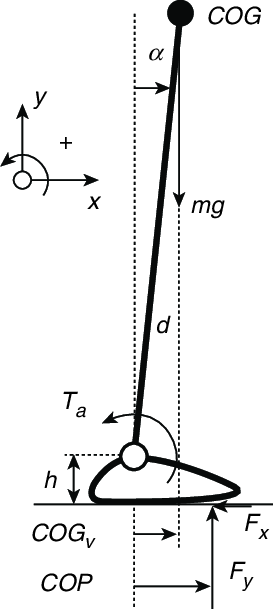
\includegraphics[width=0.3\textwidth]{figures/single_inverted_pendulum.png}}
    \caption{\label{fig:inverted_pendulum} Singolo pendolo inverso}
\end{figure}

Secondo la meccanica classica di Newton-Eulero è possibile descrivere la dinamica del sistema utilizzando la seguente equazione:
\begin{equation}
    {d^2COG\ped{v} \over dt^2} \approx {mgh \over I}(COG\ped{v}-COP)
    \label{eq:approx_cogv}
\end{equation}
dove: $COG\ped{v}$ è la proiezione del centro di gravità sul piano parallelo al terreno, $COP$ è la proiezione del centro di pressione sul piano parallelo al terreno, $h$ è la distanza tra la caviglia e il baricentro e $I$ è il momento d'inerzia del corpo attorno alla caviglia

Possiamo riscrivere l'equazione \ref{eq:approx_cogv} anche come:
\begin{equation}
    {COG\ped{v}(\omega) \over COP(\omega)} = {\omega\ped{0}^2 \over \omega^2+\omega\ped{0}^2}
    \label{eq:cogv_polar}
\end{equation}
dove $\omega$ rappresenta la frequenza angolare e $w\ped{0} = \sqrt{mgh \over I}$ è la frequenza naturale del pendolo inverso. Si noti che all'aumentare della frequenza l'output del sistema diminuisce gradualmente seguendo il comportamento di un filtro passa basso; la proiezione del centro di gravità nel dominio della frequenza può essere considerata come una versione filtrata del centro di pressione.

{\itshape Infine è importante ricordare che il processo di modellizzazione del corpo umano come un singolo pendolo inverso è tutt'altro che completo, specialmente per quanto riguarda la coordinazione e i modelli di controllo; fra i tentativi di miglioramento dell'accuratezza dei modelli troviamo il doppio pendolo inverso.}

\section{Dati ottenuti dall'analisi}
Tipicamente dall'esame stabilometrico si producono due tipi di grafico (esempio in Figura \ref{fig:statokinesigramma}):
\begin{itemize}    
    \item lo {\bfseries statokinesigramma}, detto anche sway-path, raffigura lo spostamento del $COP$ nel piano $xy$
    \item lo {\bfseries stabilogramma} mostra la variazione del $COP$ nel tempo
\end{itemize}

Il $COP$ è espresso sotto forma di vettore in due dimensioni: {\bfseries\itshape Antero-Posteriore} ({\itshape AP}) e {\bfseries\itshape Medio-Laterale} ({\itshape ML}).

\begin{figure}[!htb]
    \center{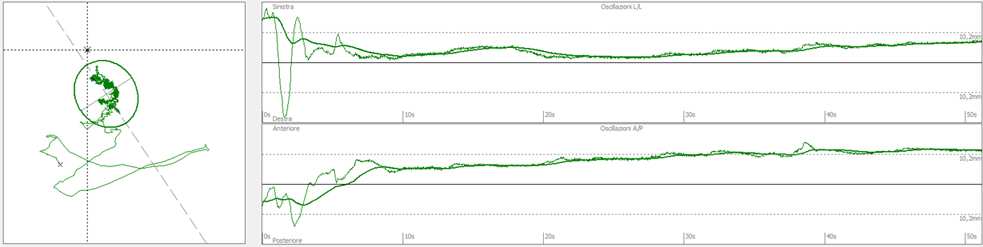
\includegraphics[width=\textwidth]{figures/statokinesigramma.jpg}}
    \caption{\label{fig:statokinesigramma} Esempio di statokinesigramma (sulla sinistra) e di stabilogramma (sulla destra)}
\end{figure}

Dallo statokinesigramma possiamo estrarre diversi parametri utili, questi possono essere classificati in due categorie: {\bfseries parametri globali} e {\bfseries parametri strutturali}; i primi studiano lo sway-pattern nella sua totalità, mentre i secondi si concentrano nel suddividere le traiettorie in pezzetti più piccoli ed estrarre da essi dati utili.

Prima di tutto è importante ricordare che lo scopo di questa tesi è lo sviluppo di un'applicazione per smartphone in grado di determinare la postura e per fare ciò i dati del COP sono ricavati partendo dai valori dell'accelerometro presente nel dispositivo; ci concentreremo solo su alcuni parametri delineando le features da calcolare come:
\begin{enumerate}
    \item Features nel dominio del tempo
    \item Features nel dominio della frequenza
    \item Features strutturali
    \item Features giroscopiche
\end{enumerate}

Le {\itshape features nel dominio del tempo} contengono tutti i parametri ricavati dallo studio del comportamento dello sway-path nel tempo: 
\begin{itemize}
    \item Sway path -> lunghezza della traiettoria del $COP$ nel tempo
    \item Mean distance -> distanza media dal centro del $COP$
    \item Standard deviation of the displacement -> deviazione standard del displacement totale del $COP$
    \item Range -> massima distanza tra due punti del $COP$
\end{itemize}

Le {\itshape features nel dominio della frequenza} si ricavano dalla frequenza dello sway-path, il loro scopo principale è quello di avere una stima dell'energia dello sway-path e di come essa è concentrata nelle varie frequenze:
\begin{itemize}
    \item Frequency at 80\% -> banda di frequenza che contiene l'80\% della frequenza nello spettro AP e ML
    \item Mean frequency -> media della frequenza nello spettro AP e ML
    \item Frequency peak -> i picchi della frequenza nello spettro AP e ML
\end{itemize}

Le {\itshape features strutturali} studiano la sway density curve (SDC) definita come la curva, tempo-indipendente, che per ogni istante temporale conta il numero di campioni consecutivi dello statokinesigramma all'interno di un cerchio di dato raggio. Gli indicatori ricavati sono i seguenti:
\begin{itemize}
    \item np -> numero medio di picchi nella SDC
    \item mean time -> media della distanza temporale fra due picchi della SDC
    \item std time -> deviazione standard di mean time
    \item mean peak -> durata media dei picchi della SDC
    \item sdt peak -> deviazione standard dei mean peak
    \item mean distance -> media della distanza spaziale fra due picchi della SDC
    \item std distance -> deviazione standard di mean distance
\end{itemize}

A differenza delle precedenti le {\itshape features giroscopiche} studiano diversi parametri partendo dai dati del giroscopio
\begin{itemize}
    \item Gyroscope mean -> valore medio del segnale del gyroscope negli assi x,y,z
    \item Gyroscope range -> range del segnale del gyroscope negli assi x,y,z
    \item Gyroscope variance -> varianza del segnale del gyroscope negli assi x,y,z
    \item Gyroscope kurtosis -> indice di curtosi del segnale del gyroscope negli assi x,y,z
    \item Gyroscope skewness -> indice d'asimmetria del segnale del gyroscope negli assi x,y,z
\end{itemize}
\chapter{I sensori inerziali negli Smartphone}
\label{cap:i_sensori_inerziali_negli_smartphone}

\section{Sensori presenti negli smartphone}
Dal lancio sul mercato del primo modello di IPhone nel 2007 gli smartphone hanno visto un enorme esplosione in popolarità tanto che al giorno d'oggi la maggior parte delle persone ne possiede almeno uno, che sia per uso personale o lavorativo.

Per offrire agli utenti un numero sempre crescente di funzionalità questi device fanno largo uso di sensori, montandone di tipi più disparati. I sensori più comuni sono {\bfseries l'accelerometro}, il {\bfseries giroscopio} e il gps, che consentono al device di sapere in ogni momento la sua posizione e il suo orientamento e vengono usati per i sistemi di tracking e per la rotazione automatica dello schermo; altri sensori molto diffusi negli smartphone sono: il sensore di prossimità, utilizzato per spegnere lo schermo quando l'utente avvicina il telefono all'orecchio durante una chiamata, il sensore di luminosità, che aggiusta la luminosità dello schermo in base alle condizioni di luce presenti e il lettore di impronte digitali, sempre più popolare, sta prendendo il posto delle comuni password per sbloccare il dispositivo o per convalidare le transazioni online (come i pagamenti elettronici).

Alcuni produttori di smartphone si spingono oltre, integrando sensori specifici per il monitoraggio dello stato di salute come: il termometro, il cardiofrequenzimetro, il sensore di umidità, e il pedometro (per misurare con esattezza il numero di passi compiuti dall'utente).

\begin{figure}[!htb]
    \centering
    \begin{subfigure}{0.4\textwidth}
        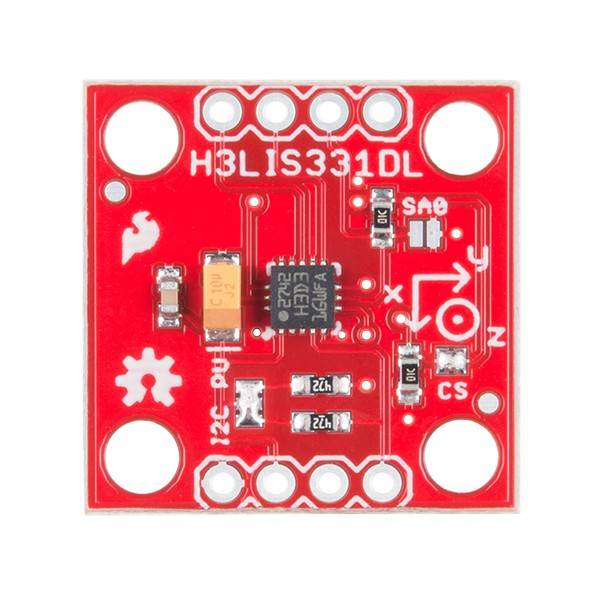
\includegraphics[width=\textwidth]{figures/accelerometer.jpg}
        \caption{Accelerometro (H3LIS331DL)}
        \label{fig:accelerometer}
    \end{subfigure}
    \begin{subfigure}{0.4\textwidth}
        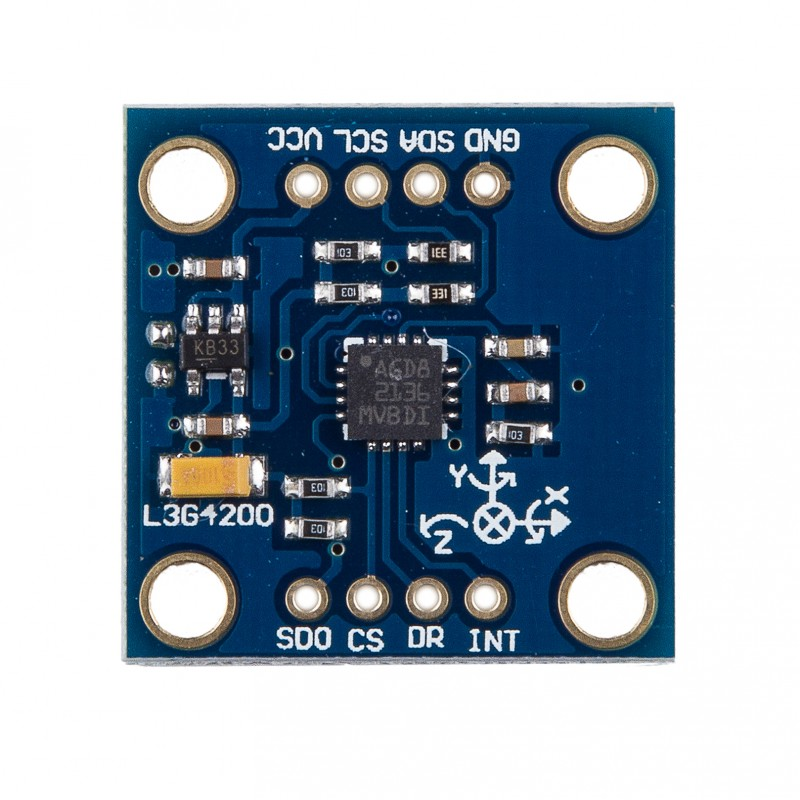
\includegraphics[width=\textwidth]{figures/gyroscope.jpg}
        \caption{Giroscopio (L3G4200D)}
        \label{fig:gyroscope}
    \end{subfigure}
    \caption{Esempio di due sensori MEMS integrati in un microchip}
    \label{fig:accelerometer_gyroscope}
\end{figure}

\section{L'accelerometro}
L'accelerometro (Figura \ref{fig:accelerometer}) è un dispositivo in grado di misurare l'accelerazione propria di un oggetto; concettualmente un accelerometro si comporta come una massa smorzata collegata ad una molla, quando il sensore risente di un'accelerazione la massa si sposta per inerzia comprimendola. Nei dispositivi commerciali spesso sono usati sensori con componenti capacitive o piezoelettriche in grado di convertire il moto della massa in un segnale elettrico comprensibile dagli strumenti di misura.

Negli ultimi anni l'uso dell'accelerometro è aumentato notevolmente a causa della sua diffusione in ambito civile, per questo con il moltiplicarsi delle applicazioni si è visto lo sviluppo di nuove tipologie di sensore, in grado di compiere misurazioni nella maniera più disparata; molti sensori lavorano in piano, ovvero sono progettati per essere sensibili solo su due assi cartesiani, per questo per creare un sensore triassale (sensibile a tutti e tre gli assi) si combinano due sensori uno perpendicolare all'altro.

Gli accelerometri più moderni spesso sono di tipo MEMS (Micro Electro-Mechanical Systems) prodotti con la stessa tecnologia utilizzata per creare i chip per questo hanno dimensioni veramente ridotte che gli consentono di integrare sullo stesso chip sia le componenti meccaniche di misurazione che quelle elettroniche di controllo. Il sensore MEMS è costituito da due condensatori dove la massa di prova è una delle due armature, quando l'accelerazione esterna sposta la massa la capacità dei condensatori varia ed è misurando questa variazione che è possibile quantificarla.

\section{Il Giroscopio}
Il giroscopio (Figura \ref{fig:gyroscope}) è un dispositivo fisico rotante inventato nel 1852 dal fisico Jean Bernard Léon Foucault; esso è costituito da un disco circolare montato su un sistema che lascia l'asse di rotazione libera di muoversi. Quando il disco è in rotazione l'orientamento del suo asse rimane parallelo e si oppone ad ogni tentativo di cambiamento in accordo con la legge di conservazione del momento angolare.

Oltre a quello meccanico esistono altri tipi di giroscopio, il giroscopio laser è composto da specchi e tubi cavi che direzionano un raggio laser in un percorso circolare e opera grazie al principio di Sagnac, il giroscopio a fibra ottica, invece, utilizza sottili fibre ottiche, mentre il giroscopio quantistico sfrutta fenomeni della meccanica quantistica per misurare l'asse di rotazione di un superconduttore; giroscopi di questo tipo sono molto precisi e stabili.

Al giorno d'oggi i giroscopi hanno svariati utilizzi dai sistemi di guida automatici per aerei, missili e sottomarini alle stedicam utilizzate per stabilizzare le macchine da presa nei film ai sistemi di guida inerziale dei satelliti.

L'effetto giroscopico è presente come effetto collaterale in tutti i dispositivi in rapida rotazione come i volani e gli hard disk per computer e deve essere tenuto in considerazione durante la progettazione.

I giroscopi MEMS, come gli accelerometri, sono dispositivi on-chip attualmente molto comuni nei dispositivi elettronici per il grande pubblico. Il primo a popolarizzare il giroscopio nell'elettronica di consumo fu Steve Jobs con il suo primo IPhone e da allora quasi ogni smartphone e tablet ne hanno integrato uno. Poiché il giroscopio permette il calcolo dell'orientamento e della rotazione spesso vengono combinati con accelerometri per riconoscere con maggior precisione i movimenti nello spazio 3D; proprio per questo sono molto diffusi anche nel mondo del gaming, integrati nei controller delle console (Dual-Shock di PlayStation, Joy-Con di Nintendo Switch) e nei sistemi di realtà virtuale (Oculus Rift, HTC Vive).
\chapter{Applicazione per analisi stabilometrica}
\label{cap:applicazione_per_analisi_stabilometrica}

\section{Precedente sviluppo per Android}
Inizialmente questa tesi prevedeva lo sviluppo di un'applicazione nativa solo per piattaforma Android, per un certo periodo di tempo si è lavorato allo sviluppo di un prototipo utilizzando il linguaggio di programmazione Java per la parte sensibile di raccolta dei dati dai sensori e il linguaggio Kotlin per tutto ciò che riguarda la grafica e l'interazione con l'utente. Si è scelto di utilizzare in maggior parte Kotlin sia perché è il linguaggio ad oggi consigliato da Google per lo sviluppo Android, sia per le sue caratteristiche che riducono di molto il tempo di sviluppo e risultano in un codice più "pulito" e facile da leggere rispetto al tradizionale Java. 

Kotlin è un linguaggio di programmazione multi-paradigma basato sulla Java Virtual Machine (JVM), ciò significa che è compatibile al 100\% con Java; in particolare è orientato verso la programmazione ad oggetti (OOP) permettendo però un pieno uso dei concetti della programmazione funzionale come ad esempio le first-class functions e l'immutabilità dei dati, molto usata nelle collezioni e nelle mappe. Una delle funzionalità più notevoli di Kotlin è il {\itshape non-null by default}, ciò significa che le variabili non possono assumere valore nullo se non specificato risparmiandoci numerosi null-check ed eliminando i tanto temuti {\itshape NullPointerException}.

Arrivati ad un buon punto nello sviluppo del prototipo Android sono stati presi in considerazione diversi fattori, il più importante era la mancanza di un corrispettivo per IOS che non richiedesse lo sviluppo di un'applicazione completa, inoltre si è vista la disponibilità di più tempo per la consegna della tesi e si è deciso di scartare il prototipo e realizzarne un altro utilizzando il framework Flutter.

\section{Flutter}
Flutter è un framework open-source creato da Google per lo sviluppo di applicazioni native iOS, Android, web e desktop partendo da un'unica codebase scritta sfruttando il linguaggio di programmazione Dart.

Il componente fondamentale di un'applicazione Flutter è il {\bfseries Flutter Engine}; scritto prevalentemente in C++, è colui che gestisce il ciclo vitale della macchina virtuale Dart oltre ad interfacciarsi con gli SDK nativi delle piattaforme e a fornire il supporto per il rendering a basso livello utilizzando la libreria grafica Skia, anch'essa sviluppata da Google.
Una particolarità molto apprezzata del Flutter Engine è la possibilità di effettuare un {\itshape "hot reload"} dell'applicazione in cui le modifiche al codice sono immediatamente pubblicate senza bisogno di un riavvio completo o un cambio di stato, riducendo di molto i tempi d'attesa durante lo sviluppo.

Ciò che differenzia Flutter dagli strumenti comunemente usati per lo sviluppo mobile (Kotlin, Swift, ecc) è il paradigma reattivo (Reactive programming) il quale si basa su stream di dati e sulla propagazione dei cambiamenti.
Flutter si avvale di un approccio dichiarativo per quanto riguarda la grafica, l'idea principale è che {\bfseries la UI è una funzione dello stato}, ovvero l'interfaccia utente è ricostruita ad ogni cambiamento di stato applicando ad esso determinate funzioni definite dai Widget. 
Un Widget ha il compito di descrivere quale sarà l'aspetto della vista partendo dalla sua configurazione attuale e dallo stato; quando lo stato cambia il widget ricrea la UI con le nuove informazioni. Il Widget può essere considerato l'atomo, l'elemento più piccolo, della programmazione in Flutter; {\bfseries in Flutter tutto è un Widget}, l'applicazione è costruita componendo widget più semplici uno con l'altro ottenendo un {\itshape Widget Tree} che descrive l'intera applicazione.

\section{Prototipo dell' interfaccia utente con Figma}
Lo sviluppo di una UI può risultare particolarmente complesso, per questo motivo al posto di realizzare l'interfaccia utente direttamente in-code, sprecando tempo ed energia utile, si è deciso di realizzare un prototipo dell'aspetto grafico e delle interazioni di base fra le diverse schermate dell'applicazione.
Il mock è stato realizzato grazie al popolare strumento di design Figma.

Figma è un'applicazione di UI/UX design basata sul browser che permette di realizzare facilmente e velocemente dei prototipi di design.

Di seguito sono riportate le schermate principali e le loro funzionalità:
\begin{itemize}
  \item Home [Figura \ref{fig:home}], come dice il nome è la prima schermata che l'utente vede appena l'applicazione è caricata, essa fornisce l'accesso alla funzionalità principale: la possibilità di eseguire un test della postura. Qui l'utente può comunicare se il test che eseguirà sarà svolto ad occhi aperti oppure chiusi e, premendo il pulsante {\itshape start test} farà appunto partire la prova.

  \item Calibrazione del dispositivo [Figura \ref{fig:calibrate}], in questa schermata l'utente può eseguire la calibrazione dei sensori presenti nel suo dispositivo; questo è fatto al fine di eguagliare l'esperienza di test fra i numerosi smartphone che montano sensori di marca e modello più disparati e che possono avere degli errori nella fasatura di fabbrica.
Durante la calibrazione l'utente è esortato ad appoggiare il suo dispositivo a "faccia in su" su una superficie piana, ad esempio un tavolo, per 10 secondi. Al termine del processo vengono generati dei bias per gli assi di ogni sensore i quali saranno poi opportunamente sottratti dai dati ricavati nei test; è importante notare che una volta calcolati i bias rimangono costanti per ogni test e possono variare solo se si riesegue la calibrazione.
La prima volta che l'applicazione è avviata l'utente sarà portato ad eseguire una prima calibrazione non appena tenterà di eseguire un test, in questo modo si è certi che il dispositivo sia calibrato.

  \item Results [Figura \ref{fig:result}], qui sono mostrate all'utente tutte le informazioni ricavate da uno specifico test.
Le diverse informazioni sono racchiuse in varie carte: la prima contiene i grafici di statokinesigramma e stabilogramma, la seconda le features nel dominio del tempo, la terza le features nel dominio della frequenza, la quarta le features strutturali e l'ultima quelle giroscopiche. Qui l'utente ha anche la possibilità di esportare l'intero test in un file formato {\bfseries json} salvato nella memoria esterna (pubblica) del suo dispositivo. Si è scelto il formato json per la sua semplicità nel rappresentare i dati e per l'ottimo supporto nativo in flutter.

  \item Durante il primo avvio l'utente non è portato subito nella home, ma in una schermata d'introduzione con diverse pagine [Figura \ref{fig:onboarding}] nelle quali si da il benvenuto all'utente, si spiega lo scopo dell'applicazione e si chiedono i dati d'anamnesi; questa parte può anche essere saltata poiché le informazioni non sono obbligatorie.
\end{itemize}

\begin{figure}
  \centering
  \begin{subfigure}[b]{0.33\textwidth}
      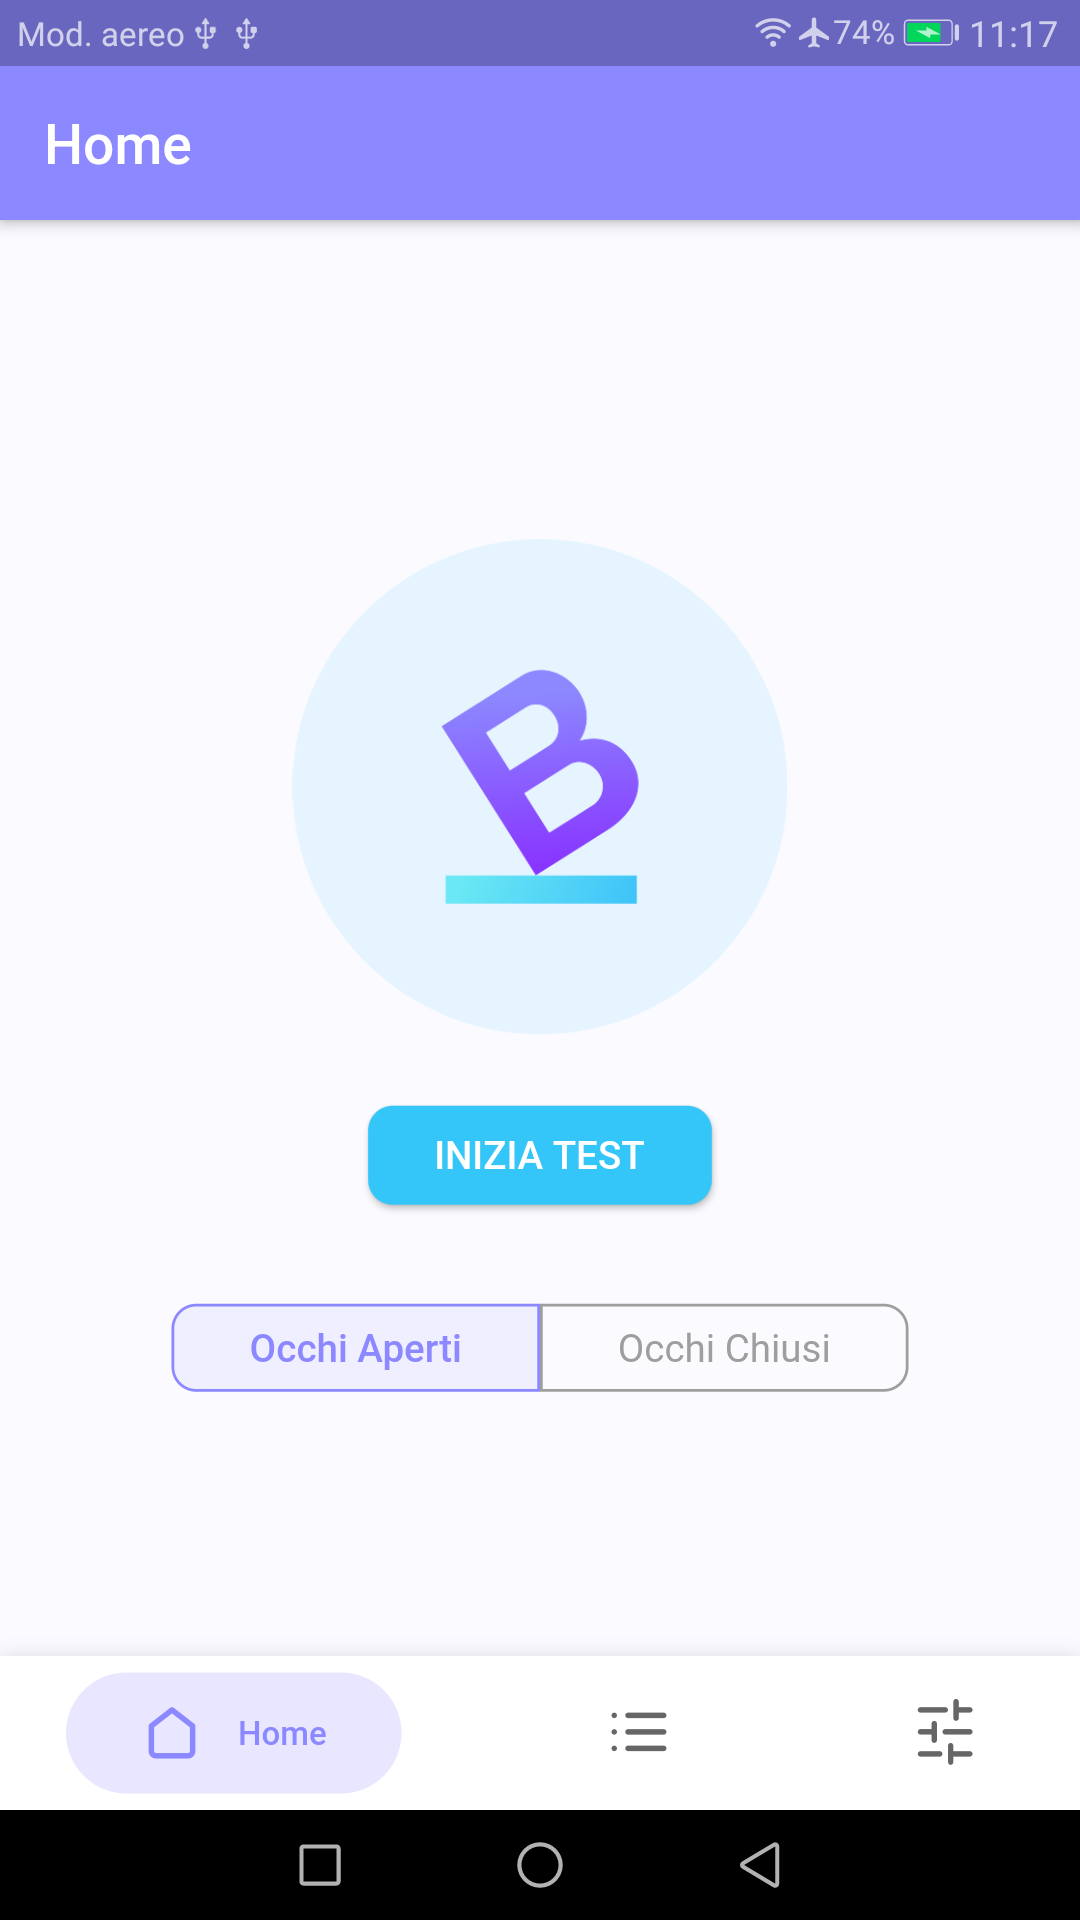
\includegraphics[width=\textwidth]{figures/screenshot/home.png}
      \caption{Pagina principale}
      \label{fig:home}
  \end{subfigure}
  \hspace{0.15\textwidth}%
  \begin{subfigure}[b]{0.33\textwidth}
      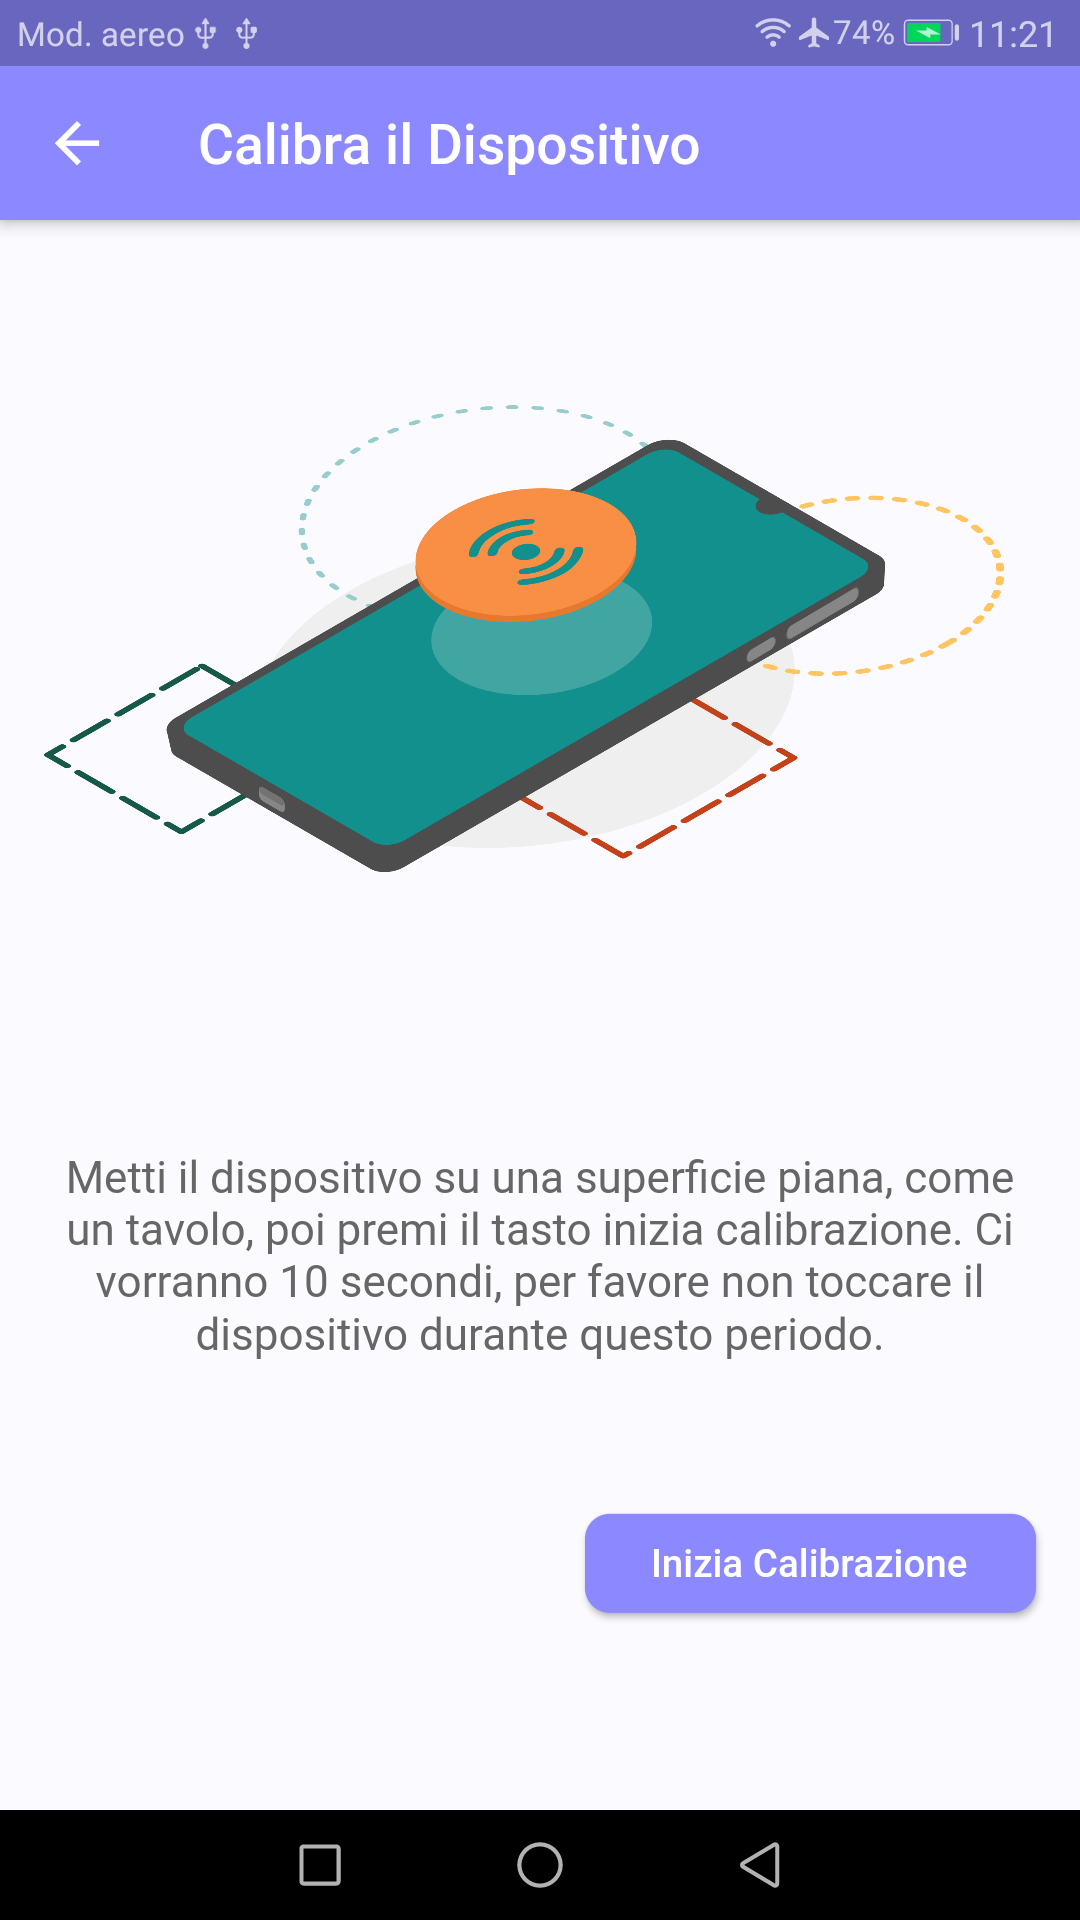
\includegraphics[width=\textwidth]{figures/screenshot/calibrate.png}
      \caption{Pagina di calibrazione del dispositivo}
      \label{fig:calibrate}
  \end{subfigure}
  \vfill
  \begin{subfigure}[b]{0.33\textwidth}
      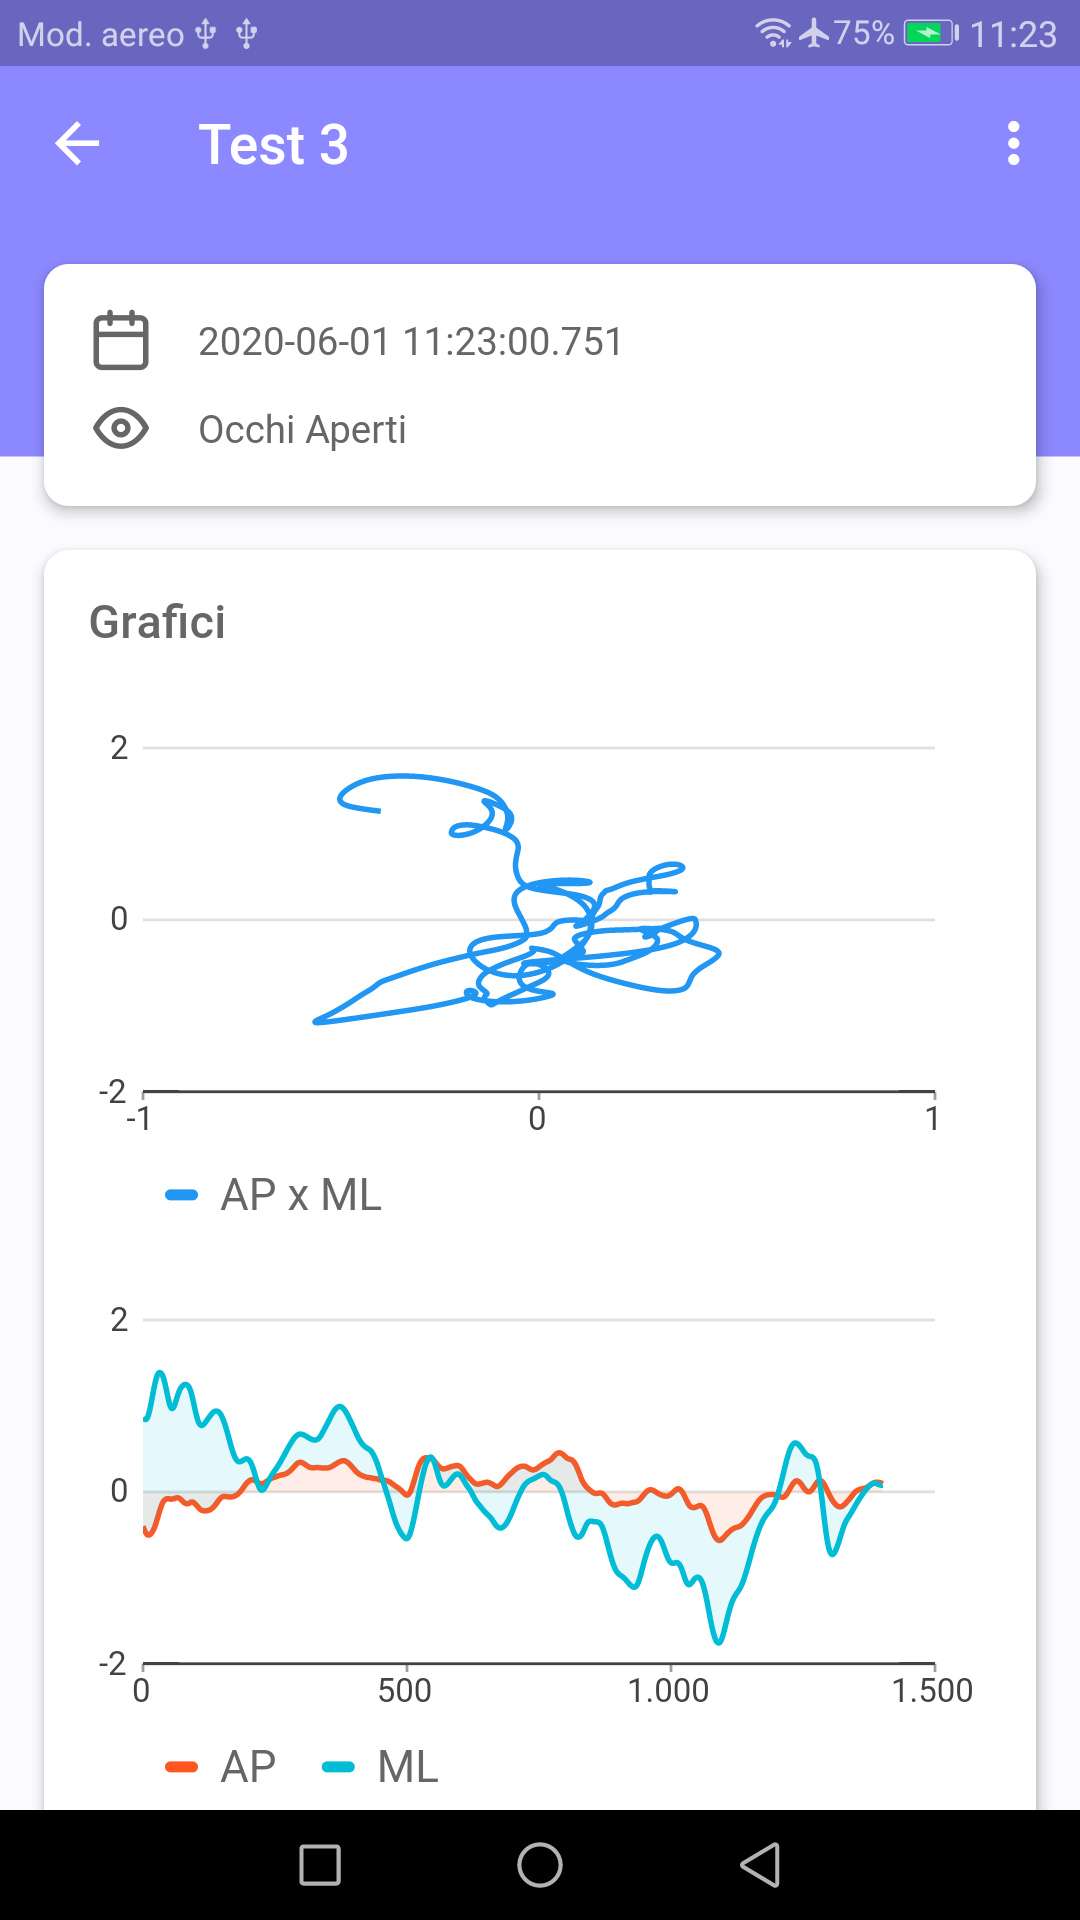
\includegraphics[width=\textwidth]{figures/screenshot/result.png}
      \caption{Pagina con i risultati di un test}
      \label{fig:result}
  \end{subfigure}
  \hspace{0.15\textwidth}%
  \begin{subfigure}[b]{0.33\textwidth}
      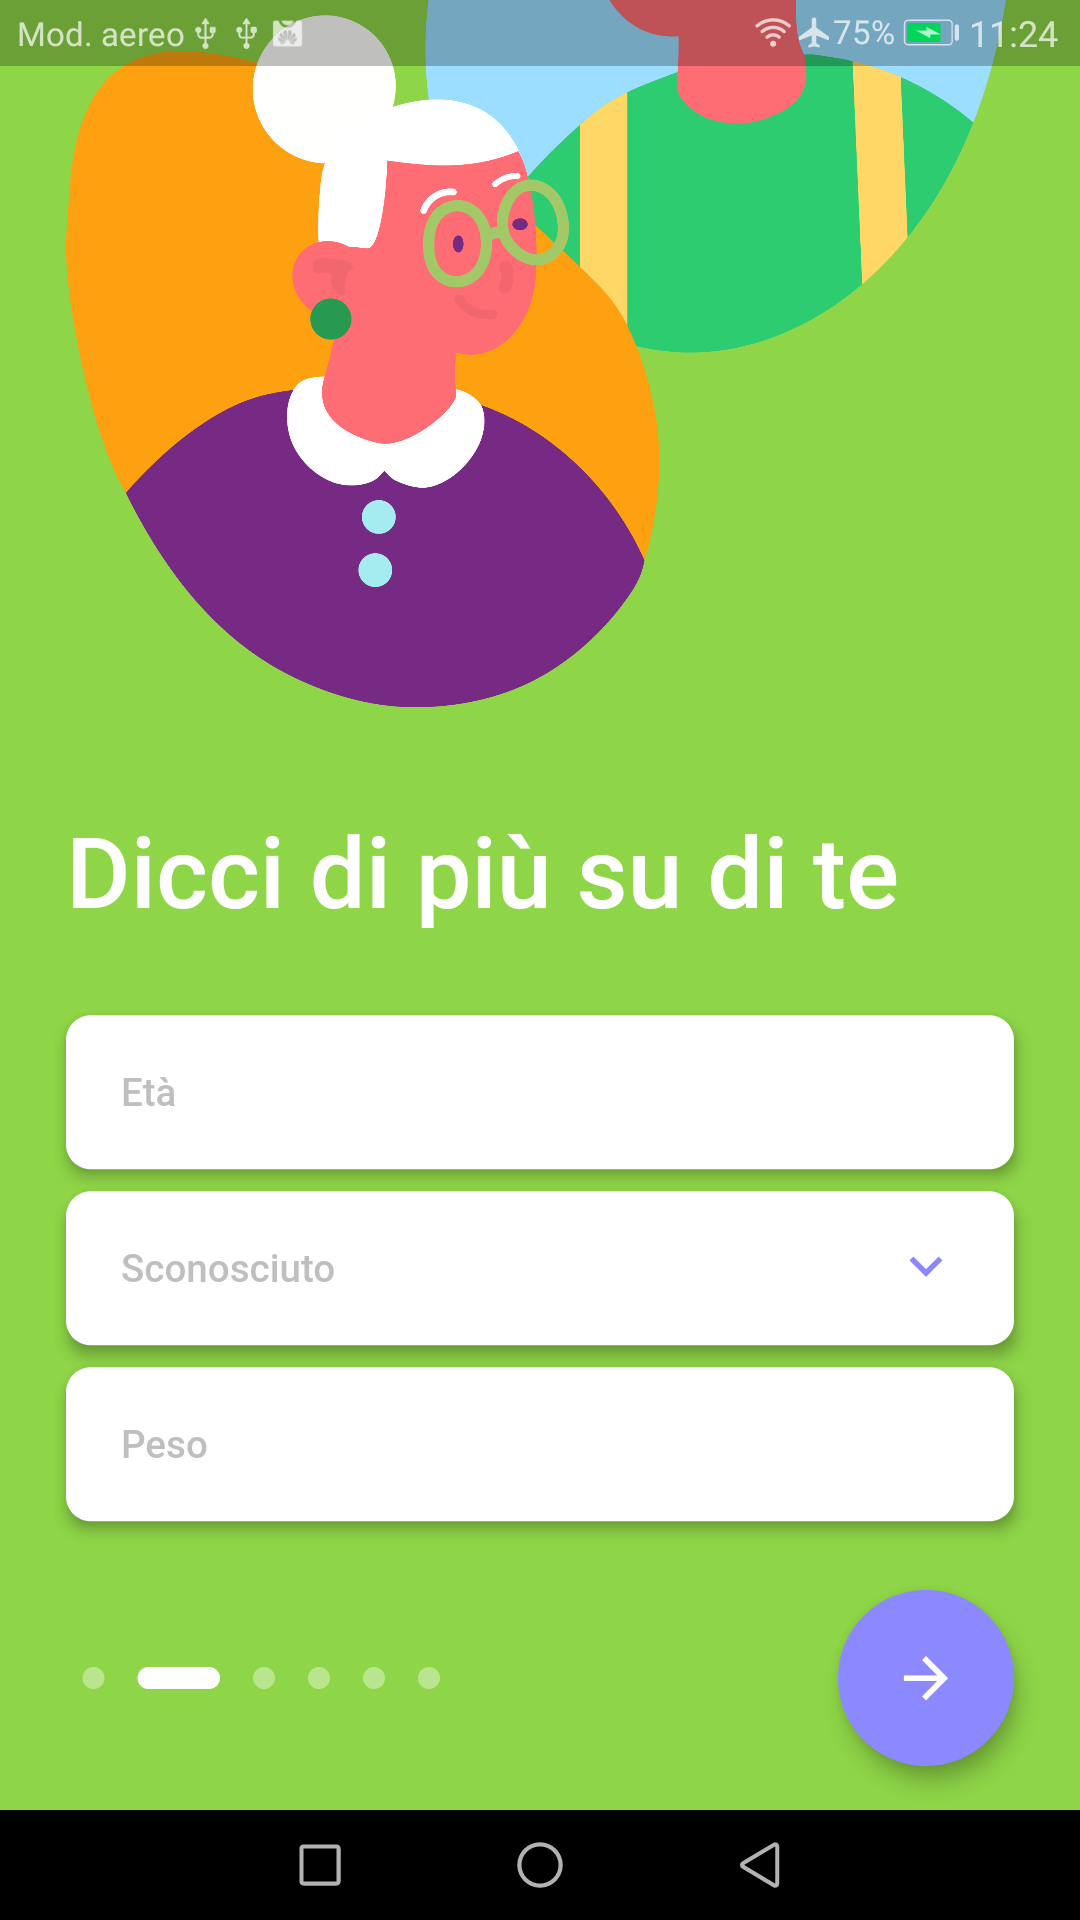
\includegraphics[width=\textwidth]{figures/screenshot/general_info.png}
      \caption{Una delle pagine in cui si chiedono i dati d'anamnesi}
      \label{fig:onboarding}
  \end{subfigure}
  \caption{Esempio di alcune delle schermate dell'applicazione}
  \label{fig:accelerometer_gyroscope}
\end{figure}

\newpage
\section{I dati d'anamnesi}
L'applicazione è progettata in modo da garantire all'utente il completo anonimato, per questa tesi si è scelto di non interfacciare l'applicazione con un database esterno, ma di salvare tutto in maniera privata all'interno del dispositivo dell'utente.

Anche se in completo anonimato all'utente vengono chieste alcune informazioni personali: la principale è la sua altezza; essa è utilizzata dall'algoritmo che estrae i COGv partendo dall'accelerometro (equazione del Capitolo \ref{cap:analisi_stabilometriche}) ed è essenziale per una corretta stima della postura. I restanti dati d'anamnesi non obbligatori sono:
\begin{itemize}
  \item l'età
  \item il genere
  \item il peso
  \item eventuali problemi posturali
  \item la presenza di problemi posturali in famiglia
  \item l'utilizzo di medicinali che possono interferire con la postura
  \item eventuali altri traumi
  \item difetti visivi
  \item difetti uditivi
\end{itemize}

Al momento all'utente è richiesta solo una piccola parte di tutti i possibili dati d'anamnesi poiché non è questo lo scopo della tesi, ma in futuro sarà possibile estenderli ed utilizzarli, assieme ai dati posturali ricavati dai vari test, per eseguire studi di correlazione.

\section{Il test della postura}
Come detto anche in precedenza lo scopo principale dell'applicazione è eseguire i test della postura, l'idea è che ogni test sia fattibile in pochi secondi e possa essere eseguito quante volte si vuole. Il test della postura si può effettuare ad occhi aperti oppure chiusi, scegliendo l'opportuna voce nella schermata home. Prima del test vero e proprio viene mostrato un contatore di 5 secondi in modo che l'utente abbia il tempo per mettersi in posizione. La postura corretta per eseguire il test è in piedi, stando più dritti possibile, guardando avanti e tenendo il dispositivo con due mani circa ad altezza ombelico.
La misurazione dei sensori vera e propria dura 32 secondi; i primi due secondi devono essere rimossi poiché possono contenere "rumore" prodotto dall'utente non ancora in posizione, questo ci lascia un campione di 30 secondi, molto simile a quello ottenuto dalle pedane stabilometriche.

\section{Plugin per la lettura dei sensori}
Un plugin in Flutter è una libreria di codice in grado di chiamare API specifiche della piattaforma, per questo esso contiene non solo codice scritto in Dart, ma anche parti di codice "nativo", scritto nel linguaggio di sviluppo della piattaforma (Kotlin/Java per Android, Swift/ObjectiveC per IOS), in questo modo è possibile ottenere più prestazioni, e utilizzare funzionalità specifiche per la piattaforma.

Per quest'applicazione in particolare, si ha il bisogno di leggere i risultati prodotti dai sensori per un periodo di tempo configurabile a priori avendo la possibilità di annullarlo prima del termine e, cosa più importante, che l'intera sequenza ottenuta abbia una frequenza di campionamento attorno a 100Hz.

Con queste specifiche in mente si è pensato di utilizzare {\bfseries sensors}\cite{sensors}, un plugin nativo di Flutter appositamente creato per ricevere tutti i dati dei sensori, purtroppo dai test effettuati al momento dello sviluppo il plugin non era in grado di produrre sequenze con sample rate maggiore di 8-10Hz, molto al disotto del target, per questo motivo si è scelto di creare da zero un plugin che risolvesse tutti i problemi.

Il plugin è sviluppato in questo modo: la classe \mintinline{dart}{SensorMonitor} è l'entry point del codice lato dart, al suo interno è presente un \mintinline{dart}{EventChannel}, un oggetto nativo di flutter con lo scopo di fare da tramite per i messaggi da e verso le piattaforme native. 
\begin{minted}{dart}
class SensorMonitor {
    static const EventChannel _defaultSensorsEventChannel = const EventChannel("uniurb.it/sensors/stream");

    /// Default constructor
    SensorMonitor([this.duration = const Duration(milliseconds: 5000)]):
    _sensorsEventChannel = _defaultSensorsEventChannel,
    _sensorsMethodChannel = _defaultSensorsMethodChannel,
    _sensorsData = [];
    
    // ...
}
\end{minted}
Quando il getter \mintinline{dart}{sensorStream} è chiamato l'EventChannel produce uno \mintinline{dart}{StreamController}. Lo StreamController ha il compito di far partire un timer per la durata settata nel costruttore, di gestire la cancellazione preventiva o al termine del countdown e di salvare in una lista i risultati ottenuti.
\begin{minted}{dart}
Stream<Duration> get sensorStream {
  _streamController ??= StreamController.broadcast(
    onListen: () {
      _sensorsData.clear();
      _sensorsStreamSubscription = _sensorsEventChannel
        .receiveBroadcastStream()
        .map((event) => eventToSensorData(event))
        .listen((event) {
          if (event != null)
            _sensorsData.add(event);
        });
      _countdownTimer = CountdownTimer(duration, Duration(milliseconds: 1000))
        ..listen((event) => _streamController.add(event.elapsed),
          onDone: () {
            // If the StreamController is not null close it
            _streamController?.close();
          }
        );
    },
    onCancel: () {
      if (_countdownTimer.isRunning)
        _countdownTimer.cancel();
      _sensorsStreamSubscription.cancel();
      _streamController = null;
    },
  );
  return _streamController?.stream;
}
\end{minted}
Il metodo \mintinline{dart}{eventToSensorData} mappa i messaggi ottenuti dalla piattaforma nativa in \mintinline{dart}{SensorData}, oggetti che rappresentano i dati di tutti i sensori.
\begin{minted}{dart}
static SensorData eventToSensorData(List event) {
  try {
    int timestamp = event[0] as int;
    int accuracy = event[1] as int;
    double accX = event[2] as double;
    double accY = event[3] as double;
    double accZ = event[4] as double;
    double gyroX = event[5] as double;
    double gyroY = event[6] as double;
    double gyroZ = event[7] as double;
    return SensorData(
      timestamp,
      accuracy,
      accX,
      accY,
      accZ,
      gyroX,
      gyroY,
      gyroZ
    );
  } catch (_) {
    return null;
  }
}
\end{minted}
Dal lato nativo, nel metodo \mintinline{kotlin}{onListen} della classe \mintinline{kotlin}{SensorMonitor} viene inizializzata una porzione di memoria condivisa, si inizia l'ascolto dei sensori ed è creata una thread pool con un singolo thread.
\begin{minted}{kotlin}
override fun onListen(arguments: Any?, events: EventChannel.EventSink?) {
  mSharedValues.reset()
  mSensorListener.startListening()
  mThreadPool = Executors.newSingleThreadExecutor()
  mThreadPool?.execute(SensorPollingRunnable(
    mUiThreadHandler,
    Runnable {
      events?.success(SensorData.mergeSensorData(
        mSharedValues.currentAccelerometerValue,
        mSharedValues.currentGyroscopeValue
      ))
    })
  )
}
\end{minted}
Il thread parallelo \mintinline{kotlin}{SensorPollingRunnable} contiene un semplice while loop nel quale esegue un \mintinline{kotlin}{Thread.sleep()} per 10 millisecondi poi prende il valore più recente di ogni sensore nella memoria condivisa e, dopo averli convertiti in una lista di numeri li invia al codice dart come massaggio attraverso l'EventChannel.

L'esempio di codice nativo viso sopra è scritto in Kotlin, non vi sono esempi da mostrare di codice per la piattaforma IOS. Lo sviluppo di codice Swift/ObjectiveC è possible da qualsiasi ambiente di lavoro in maniera gratuita, però per poter testare il corretto funzionamento è richiesto un dispositivo IOS reale oppure un emulatore il quale è disponibile solo per dispositivi apple, per questo motivo è stato lasciato come sviluppo futuro.

\section{Il calcolo delle features e il Flutter Isolate}

L'algoritmo per il calcolo delle features è composto da 3 passaggi:
\begin{enumerate}
  \item il {\itshape raw} input è convertito in liste per gli assi di accelerometro e giroscopio
  \item i valori di COGvAP e COGvML sono calcolati partendo dai dati dell'accelerometro, internamente tutti i dati sono rappresentati sotto forma di matrici per poi estrarli in due liste al termine 
  \item le features sono calcolate utilizzando i valori di COGv e del giroscopio
\end{enumerate}

L'intero algoritmo è inserito all'interno della funzione \mintinline{dart}{compute} nativa di Flutter la quale consente di eseguire l'intero codice dentro ad un Flutter Isolate. Dart è un linguaggio single thread, ciò significa che le istruzioni sono eseguite una alla volta; per ottenere asincronia si utilizza un Event Loop. Nel caso occorra eseguire operazioni molto lente o pesanti il Flutter Isolate consente di ottenere un diverso Event Loop nel quale eseguire il codice di fatto in maniera parallela al precedente. Gli Isolate, come dice il nome, sono spazi di memoria isolati, con i quali è possibile scambiare dati solo tramite messaggi.

\section{Contributi all'Open Source}

{\bfseries Pub} è il package manager del linguaggio Dart, contenente librerie e pacchetti riusabili per Dart e Flutter; qui chiunque può sviluppare e pubblicare il proprio pacchetto o utilizzare quelli degli altri nei suoi progetti come dipendenze. Un pacchetto solitamente è un insieme di file e classi che risolvono uno specifico problema o aggiungono una determinata funzionalità.

Durante lo sviluppo dell'applicazione si è notato varie volte che alcune funzionalità potevano essere estratte come dipendenze esterne, così si è colta l'occasione per creare diversi pacchetti e pubblicarli su pub.dev 
\begin{itemize}
  \item custom\_dropdown\cite{cudropdown} fornisce una semplice dropdown con uno stile diverso da quello di default
  \item iirjdart\cite{iirjdart} è il porting in dart della libreria iirj scritta in java. Questo pacchetto fornisce le funzionalità di filtro passa alto, passa basso, passa banda ed elimina banda di tipo Butterworth, Bessel e Chebychev di tipo 1 e 2.
  \item powerdart\cite{powerdart} è un pacchetto dart per stimare la densità spettrale di potenza(PSD) ed analizzarne i risultati. Al suo interno sono presenti metodi per il calcolo della PSD e per il calcolo integrale utilizzando il metodo dei trapezi.
  \item about\_dependencies\cite{abtdependencies} ha l'obbiettivo di generare un file dart con all'interno la lista di tutte le dipendenze utilizzate nel progetto e le loro informazioni base (versione, descrizione). Questo pacchetto è particolare perché, a differenza delle altre dipendenze che vengono utilizzate dall'applicazione, questa è impiegata solo durante la fase di sviluppo ed è il file generato a far parte dell'applicazione finale.
\end{itemize}
\chapter{Test e Risultati}
\label{cap:test_e_risultati}

L'applicazione è stata testata su molti dispositivi Android di diverse marche e con differenti versioni del sistema operativo; i due smartphone utilizzati principalmente durante lo sviluppo sono: Huawei Nova Plus con Android 7 e Xiaomi Redmi Note 8T con Android 9. Come detto anche nel precedente capitolo il testing su IOS è oggetto di sviluppi futuri dunque d'ora in avanti la tesi farà riferimento solo alla versione Android dell'applicazione.

\section{Casi d'uso}

Di seguito sono riportati i diversi casi d'uso dell'applicazione (Figura \ref{fig:use_case})

\begin{figure}[!htb]
    \centering
    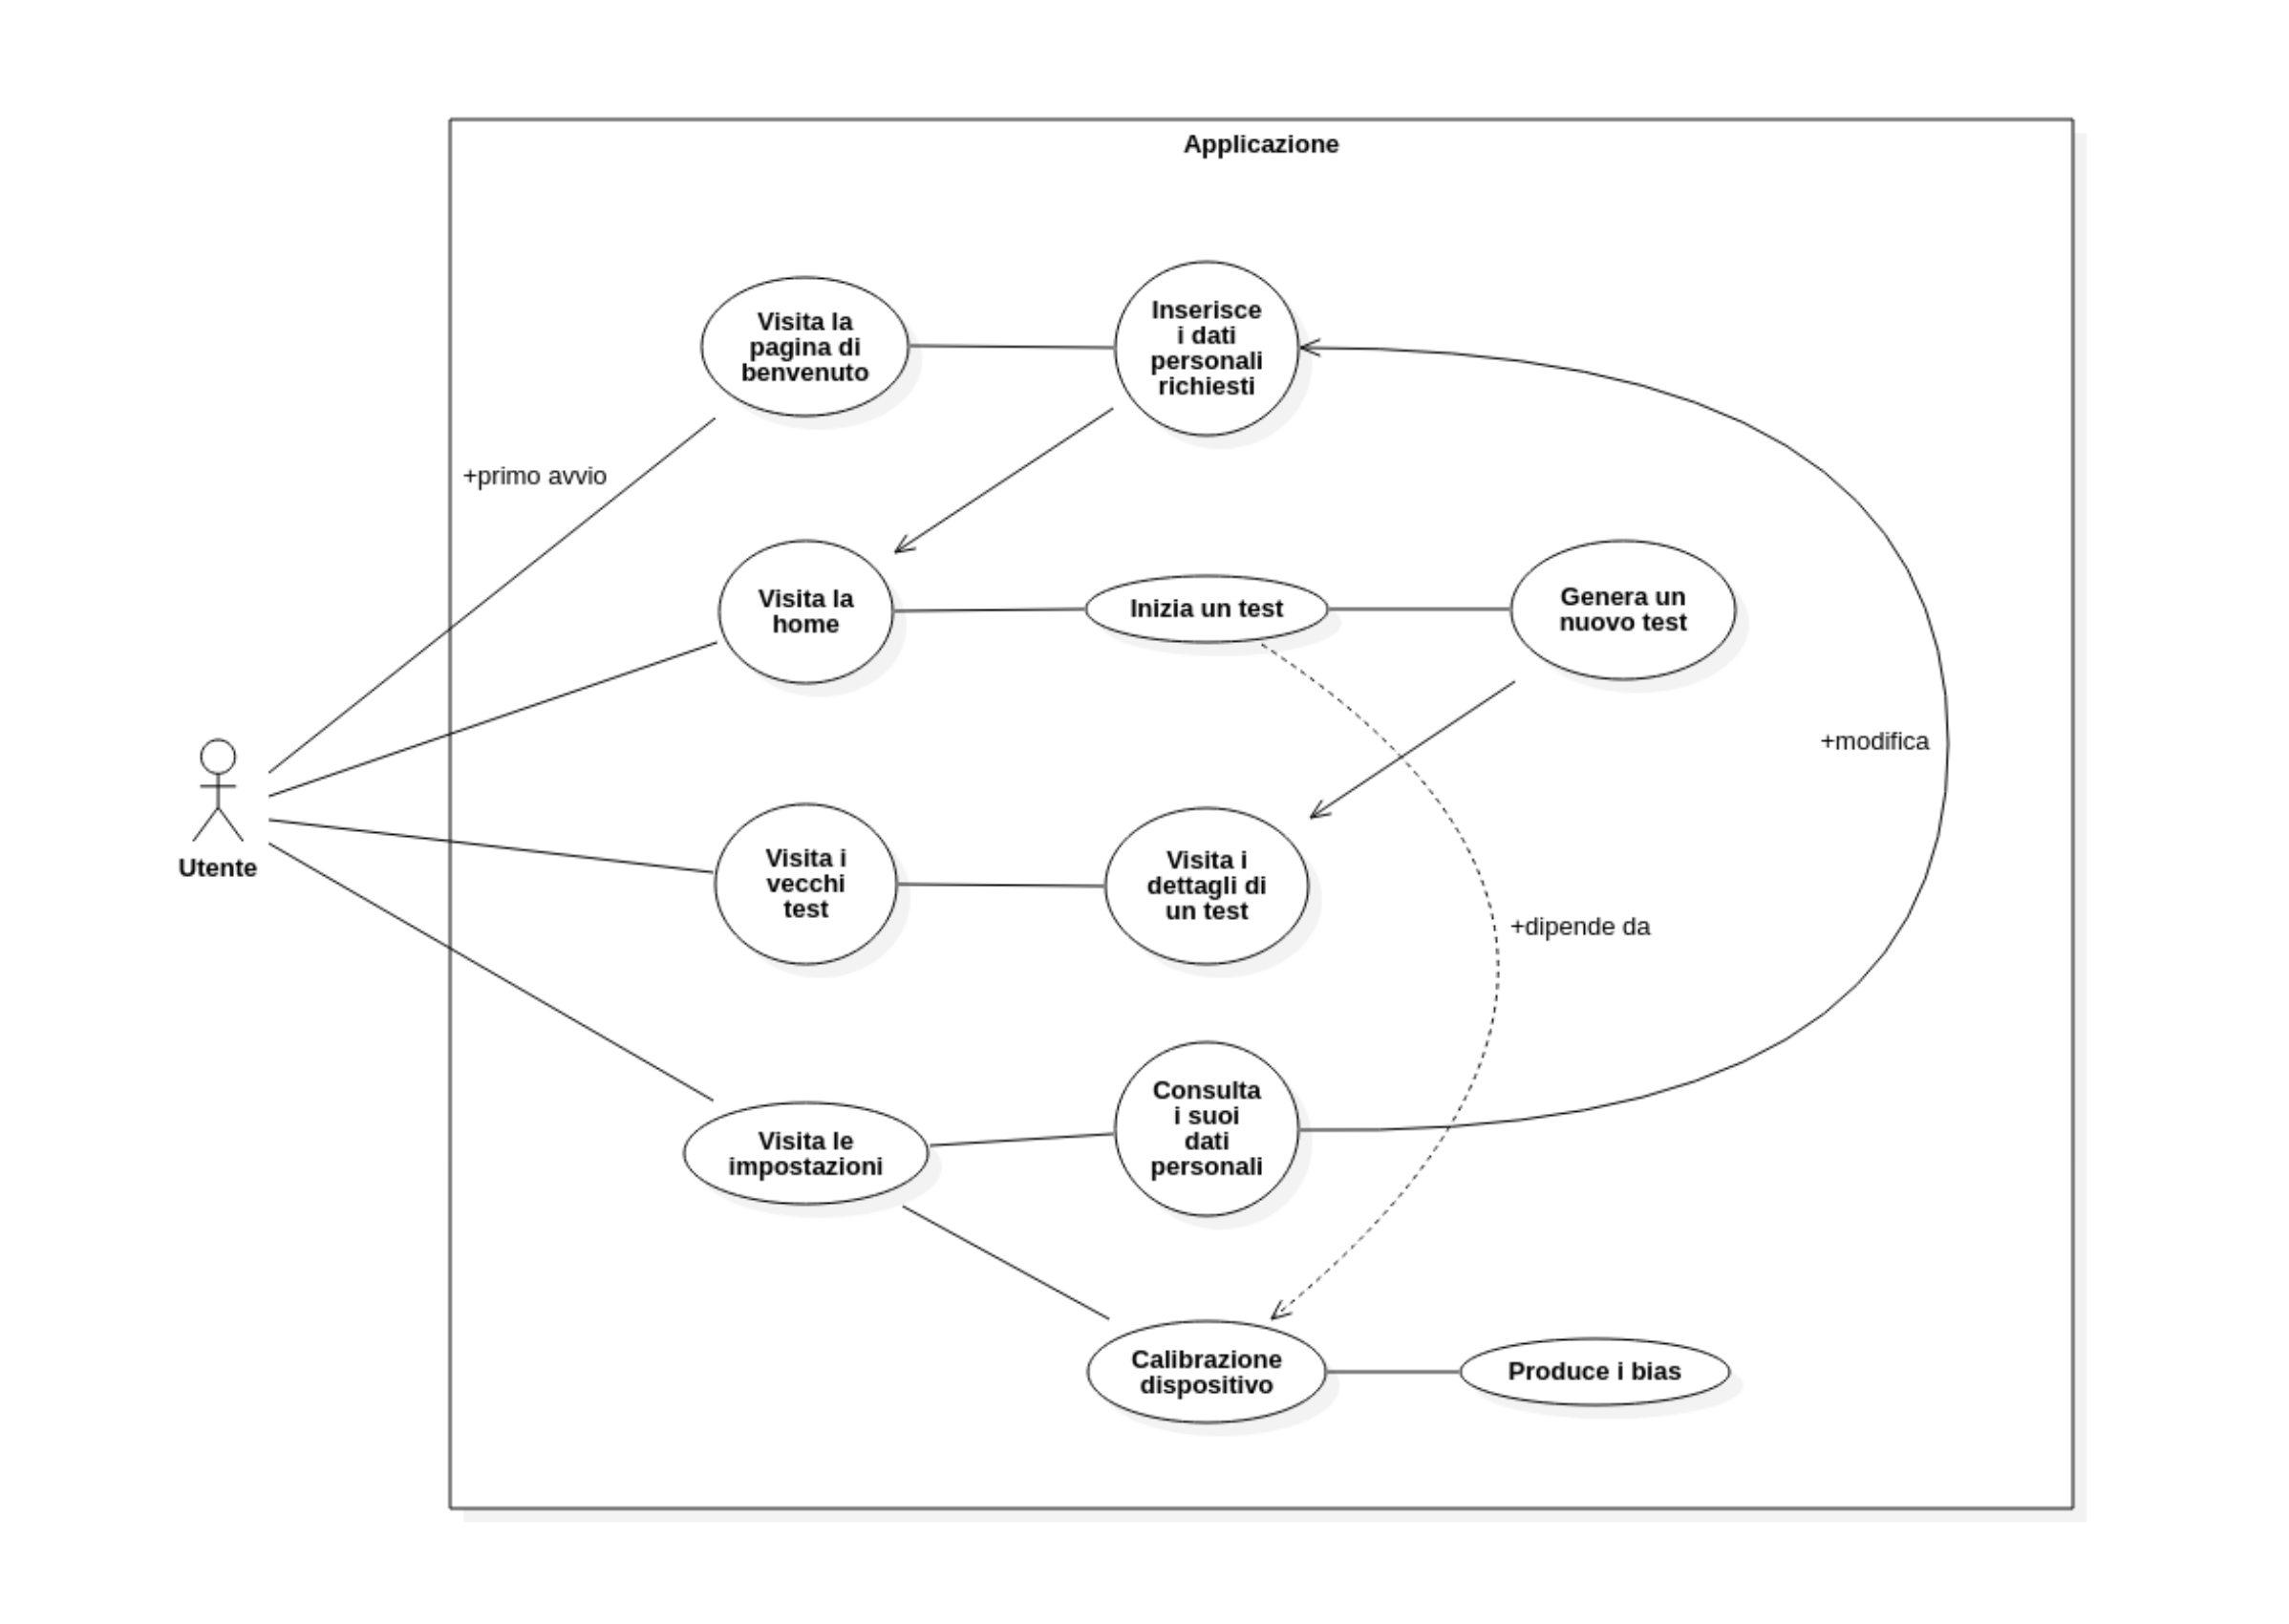
\includegraphics[width=\textwidth]{figures/use_case_diagram.png}
    \caption{Diagramma dei casi d'uso dell'intera applicazione}
    \label{fig:use_case}
\end{figure}

\subsection{primo avvio}
Durante il primo avvio l'utente è portato in una schermata di onboarding dove passa attraverso diverse pagine (Figura \ref{fig:onboarding}). Inizialmente si dà il benvenuto all'utente nell'applicazione, in seguito sono chiesti i suoi dati d'anamnesi impiegando una differente schermata per ogni categoria. I dati d'anamnesi sono divisi in:
\begin{itemize}
    \item Altezza
    \item Informazioni generali
    \item Problemi posturali
    \item Precedenti traumatici
    \item Difetti visivi/uditivi
\end{itemize}

\begin{figure}[!htb]
    \centering
    \begin{subfigure}{0.35\textwidth}
        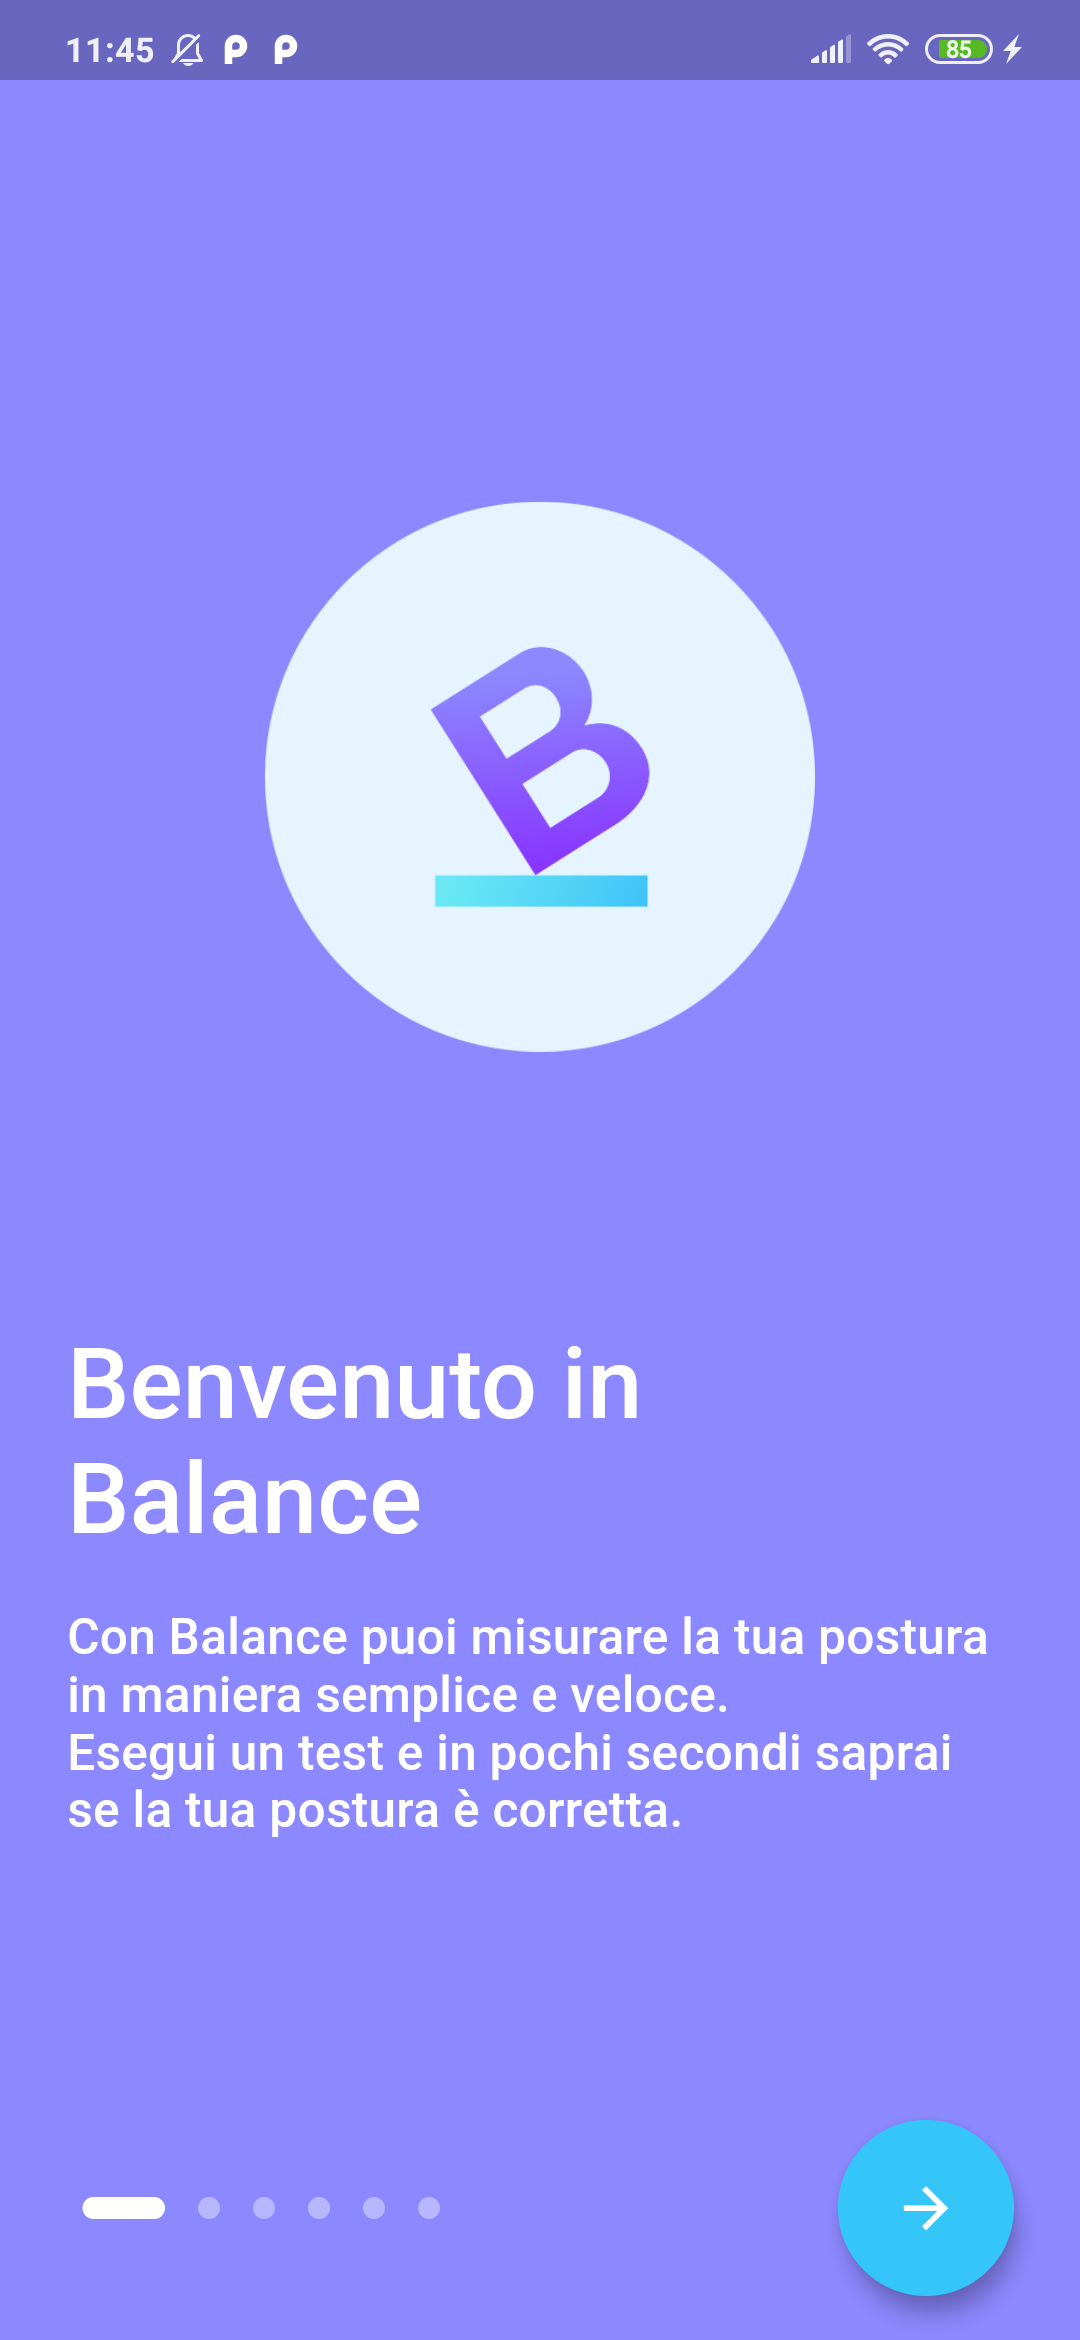
\includegraphics[width=\textwidth]{figures/screenshot/redmi_note_8t/welcome.png}
    \end{subfigure}
    \begin{subfigure}{0.35\textwidth}
        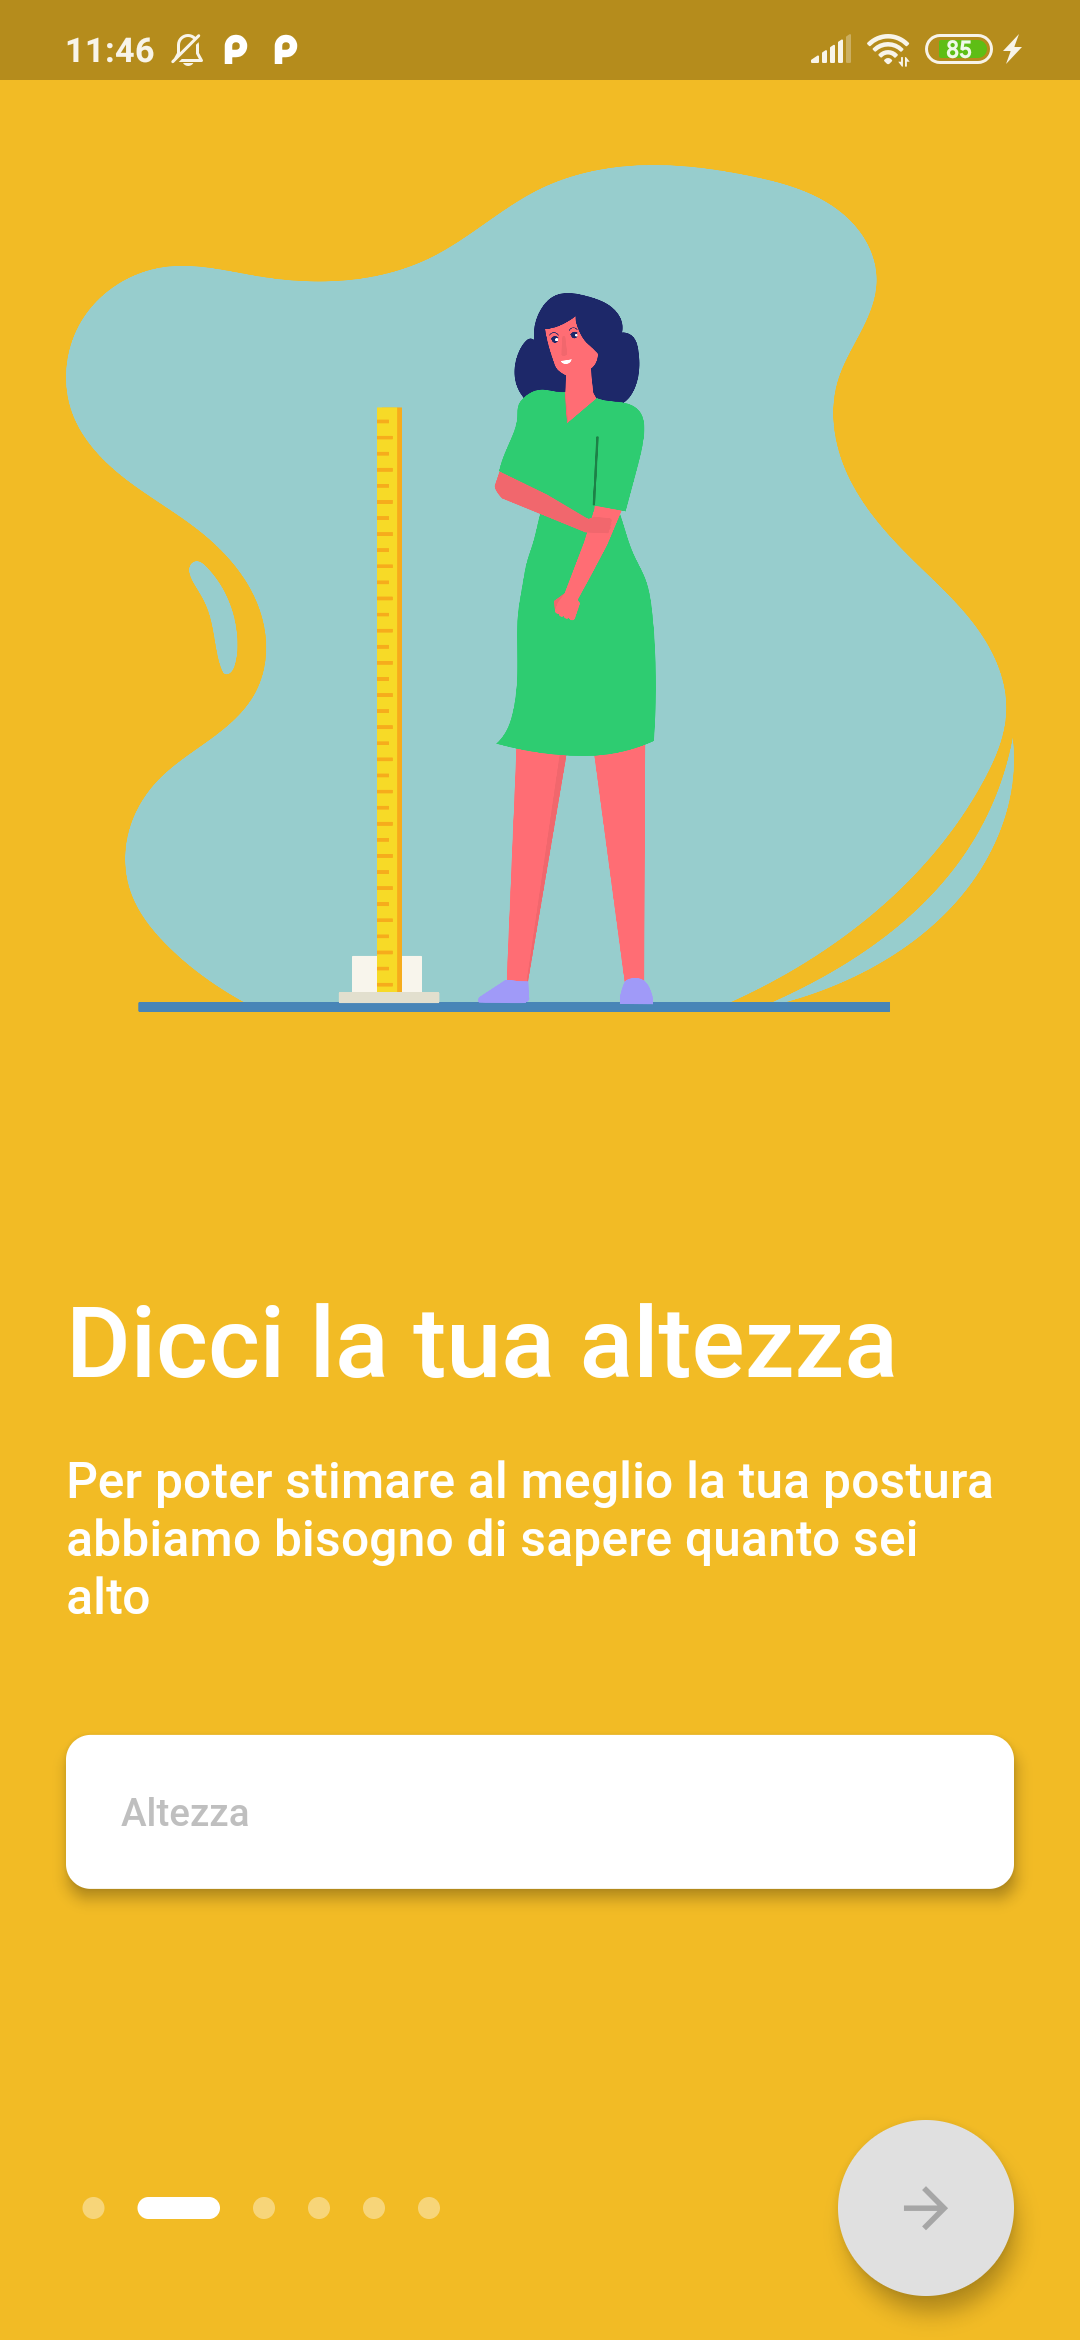
\includegraphics[width=\textwidth]{figures/screenshot/redmi_note_8t/height.png}
    \end{subfigure}
    \begin{subfigure}{0.35\textwidth}
        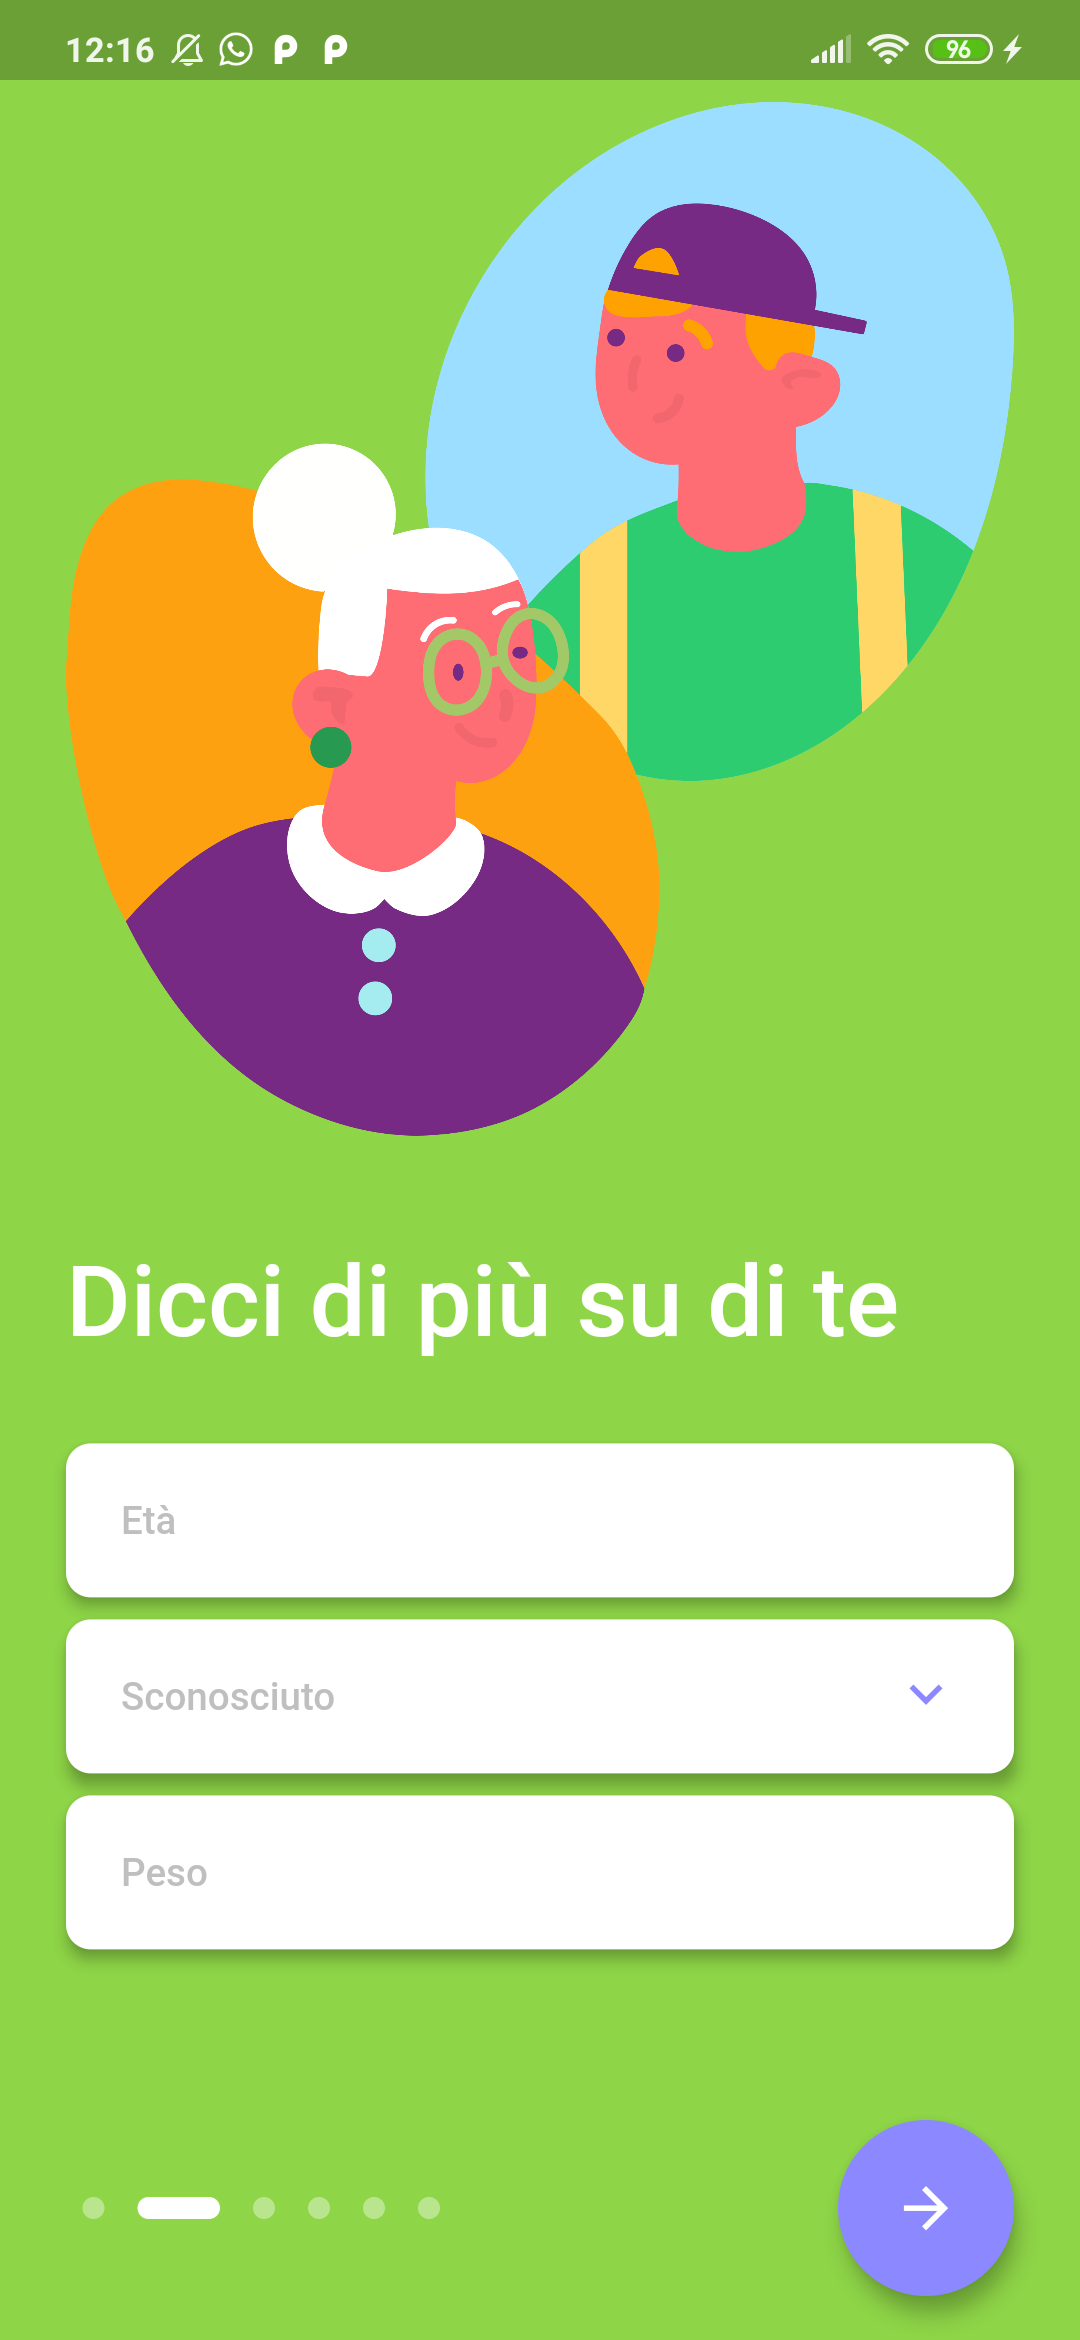
\includegraphics[width=\textwidth]{figures/screenshot/redmi_note_8t/general_info.png}
    \end{subfigure}
    \caption{Schermate di onboarding}
    \label{fig:onboarding}
\end{figure}

\subsection{home e misurazione della postura}
Dopo il primo avvio, ogni volta che l'utente aprirà l'applicazione vedrà questa pagina per prima (Figura \ref{fig:home}); questo per dare rapido accesso alla funzionalità principale: eseguire un nuovo test. Per iniziare la misurazione l'utente deve premere il bottone {\bfseries inizia test}, immediatamente apparirà un timer della durata di 5 secondi (Figura \ref{fig:home_premeasure}), dopo questo tempo, utile per mettersi in posizione, inizierà la misurazione vera e propria dei sensori (Figura \ref{fig:home_measure})

\begin{figure}[!htb]
    \centering
    \begin{subfigure}{.35\textwidth}
        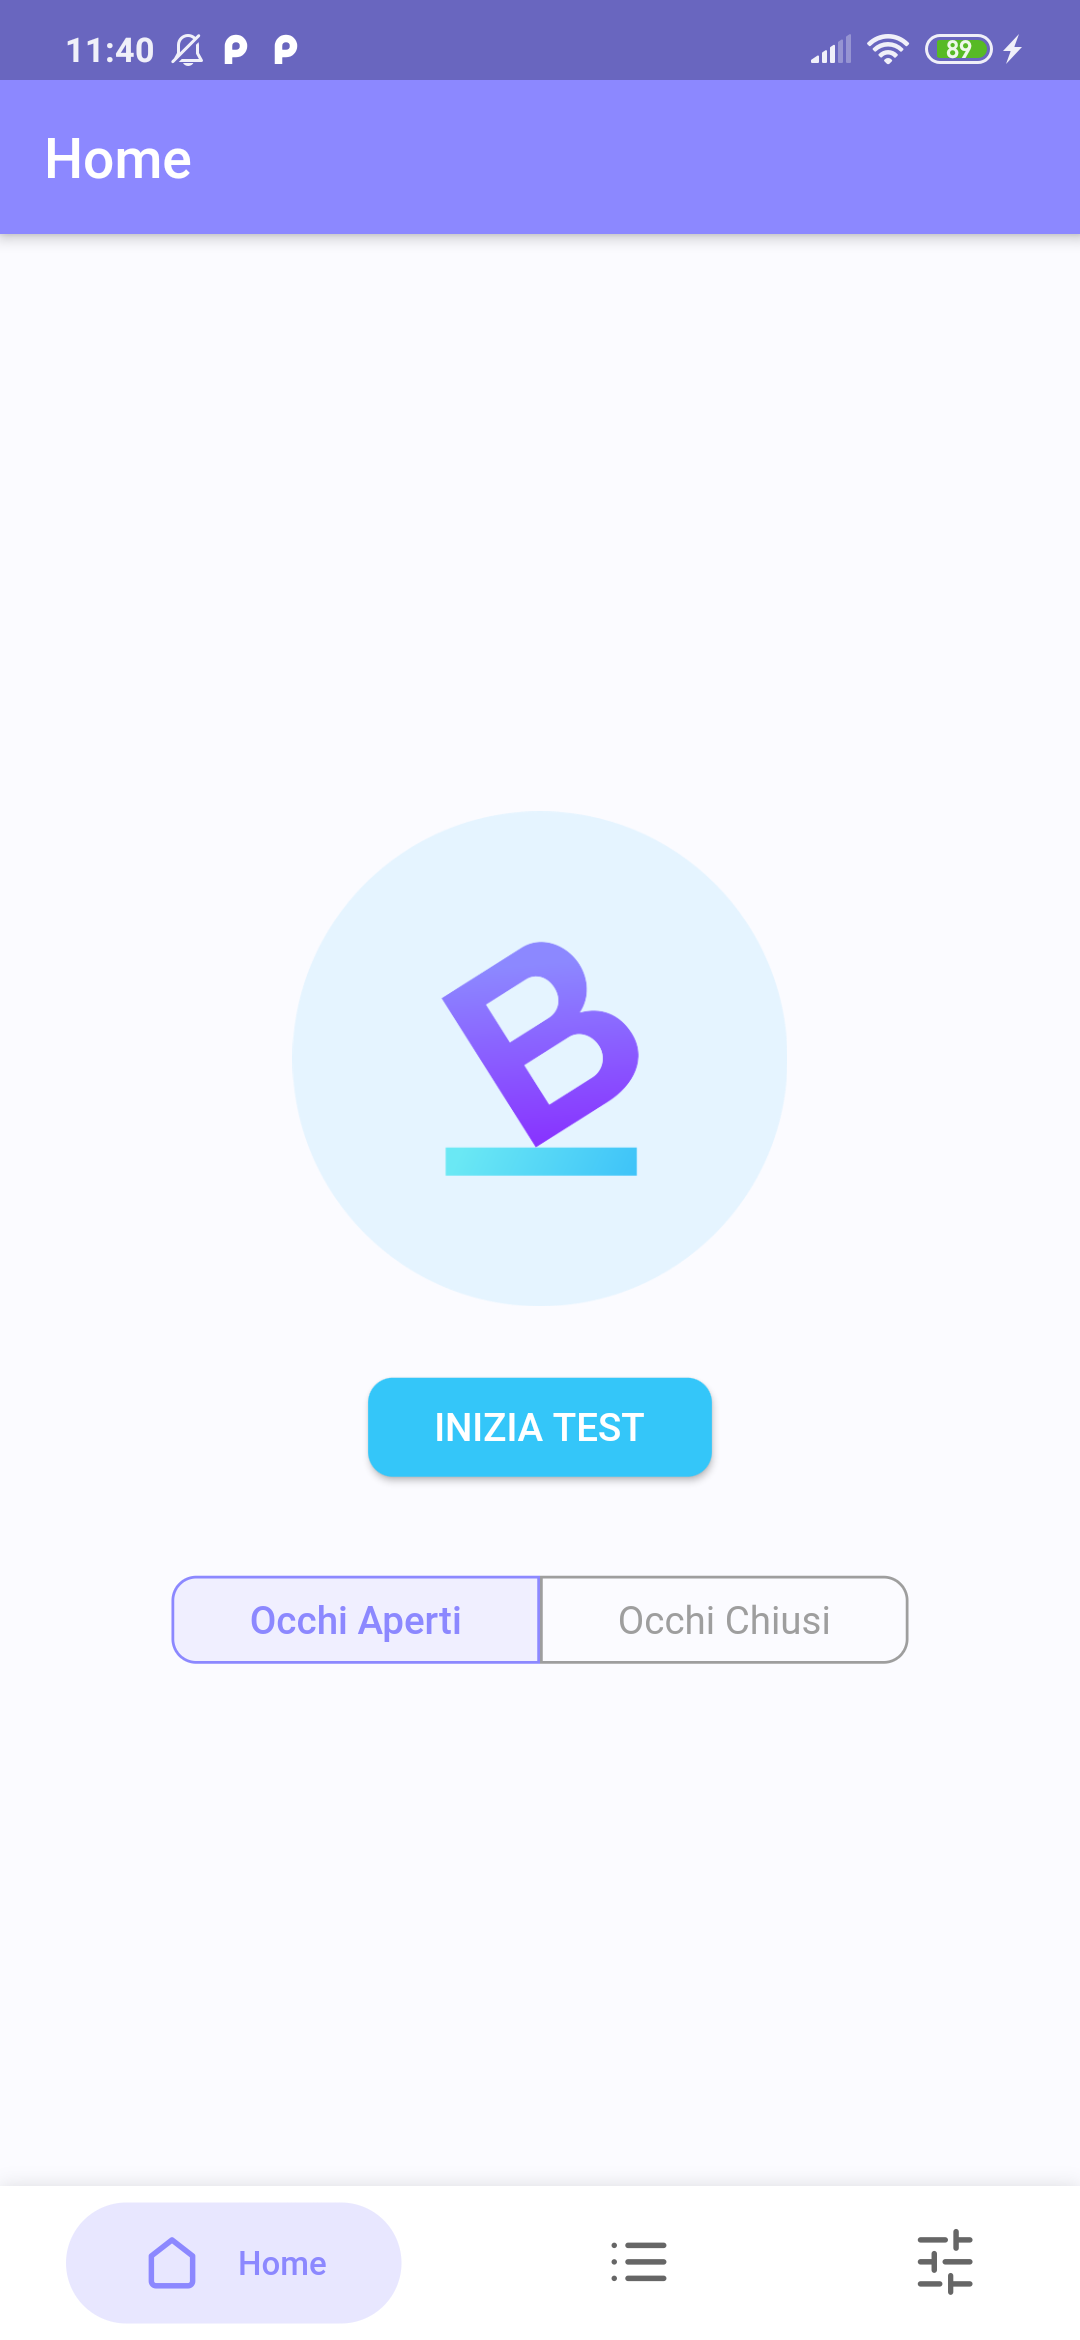
\includegraphics[width=\textwidth]{figures/screenshot/redmi_note_8t/home.png}
        \caption{allo stato iniziale}
        \label{fig:home}
    \end{subfigure}
    \hspace{.15\textwidth}%
    \begin{subfigure}{.35\textwidth}
        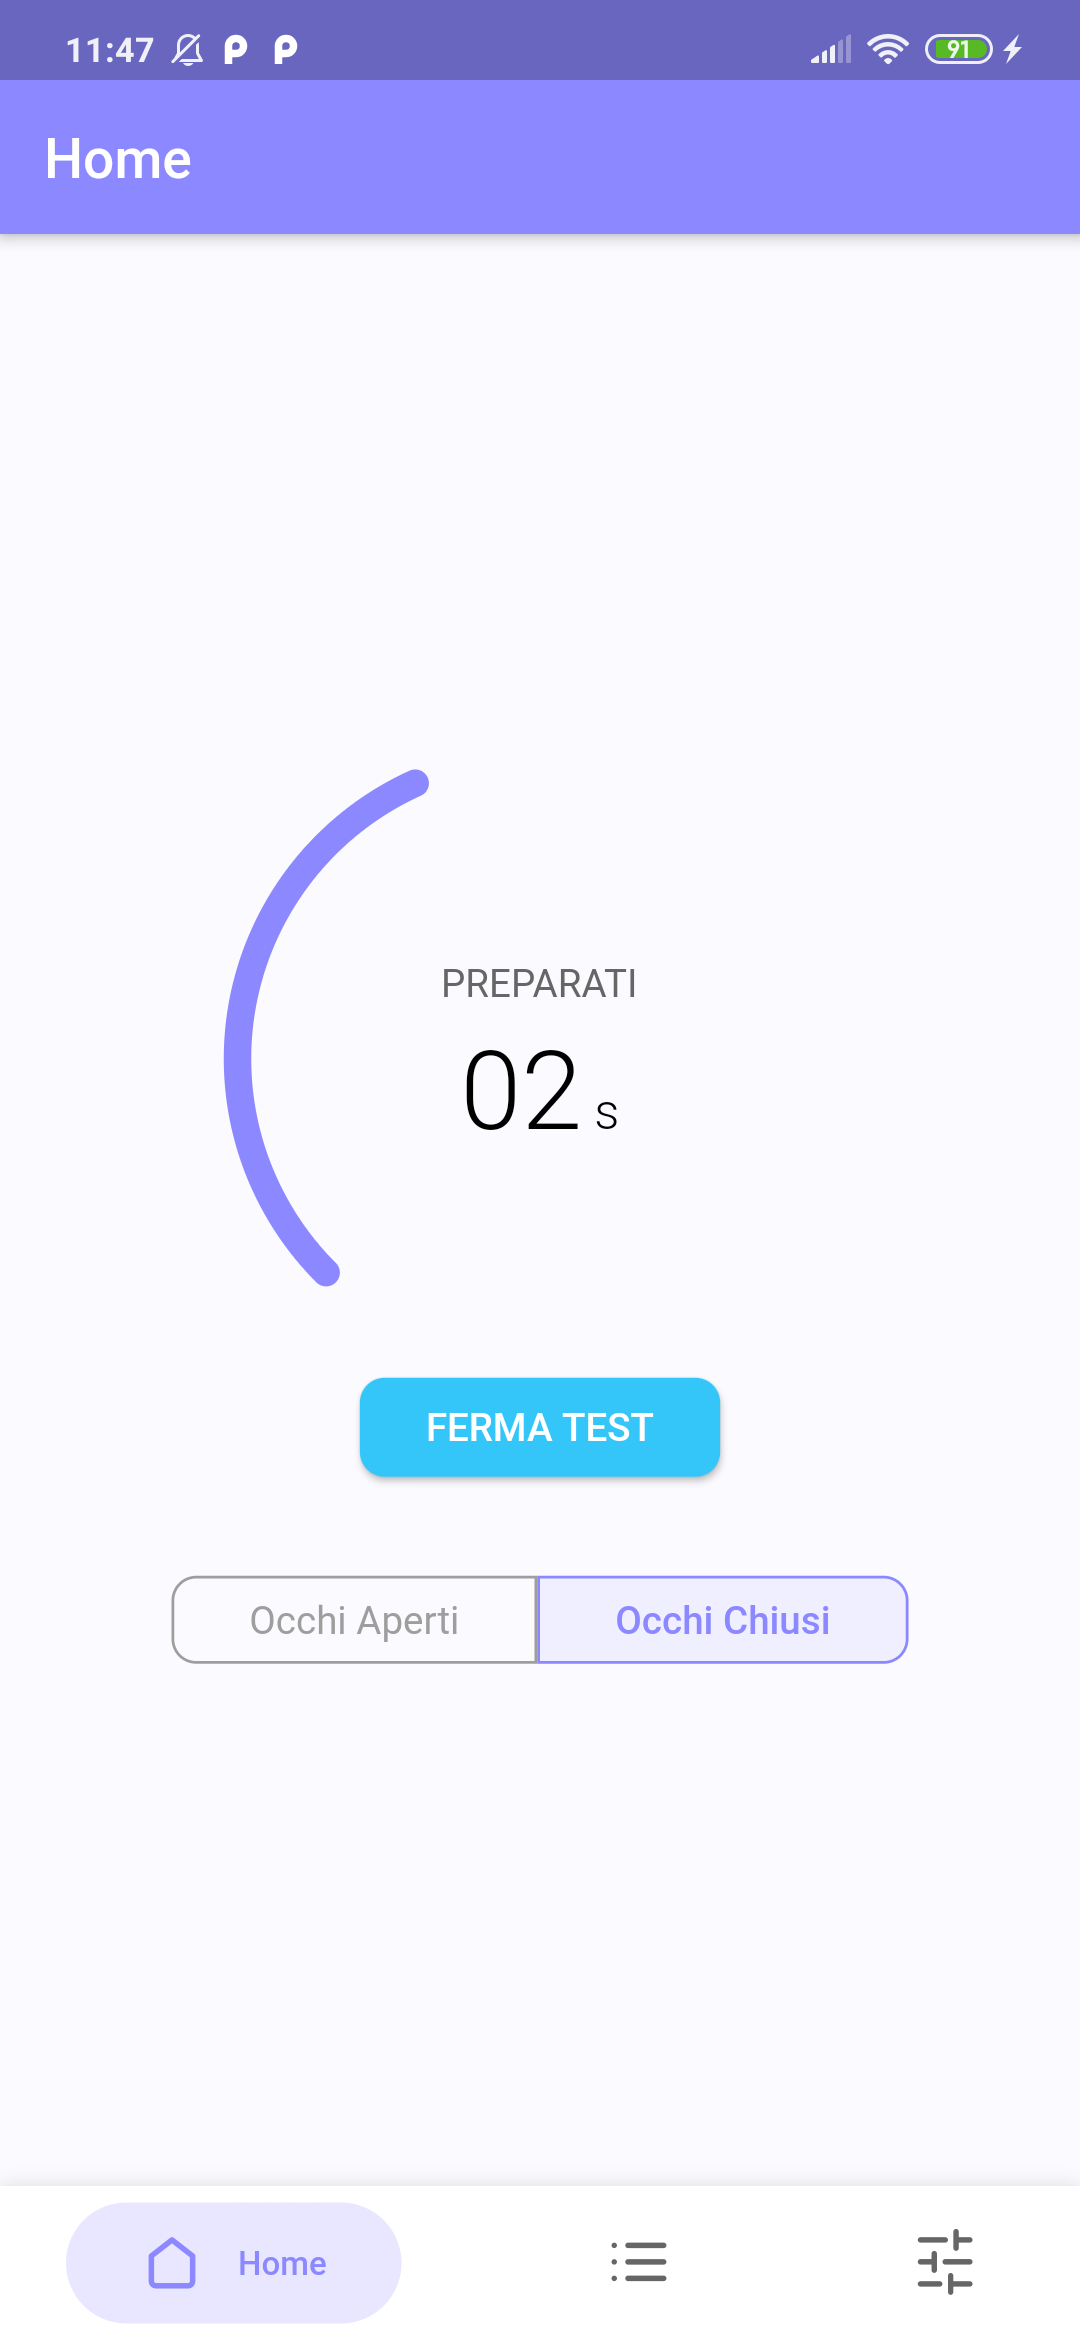
\includegraphics[width=\textwidth]{figures/screenshot/redmi_note_8t/home_measure.png}
        \caption{con il timer di 5 secondi prima della misurazione}
        \label{fig:home_premeasure}
    \end{subfigure}
    \begin{subfigure}{.35\textwidth}
        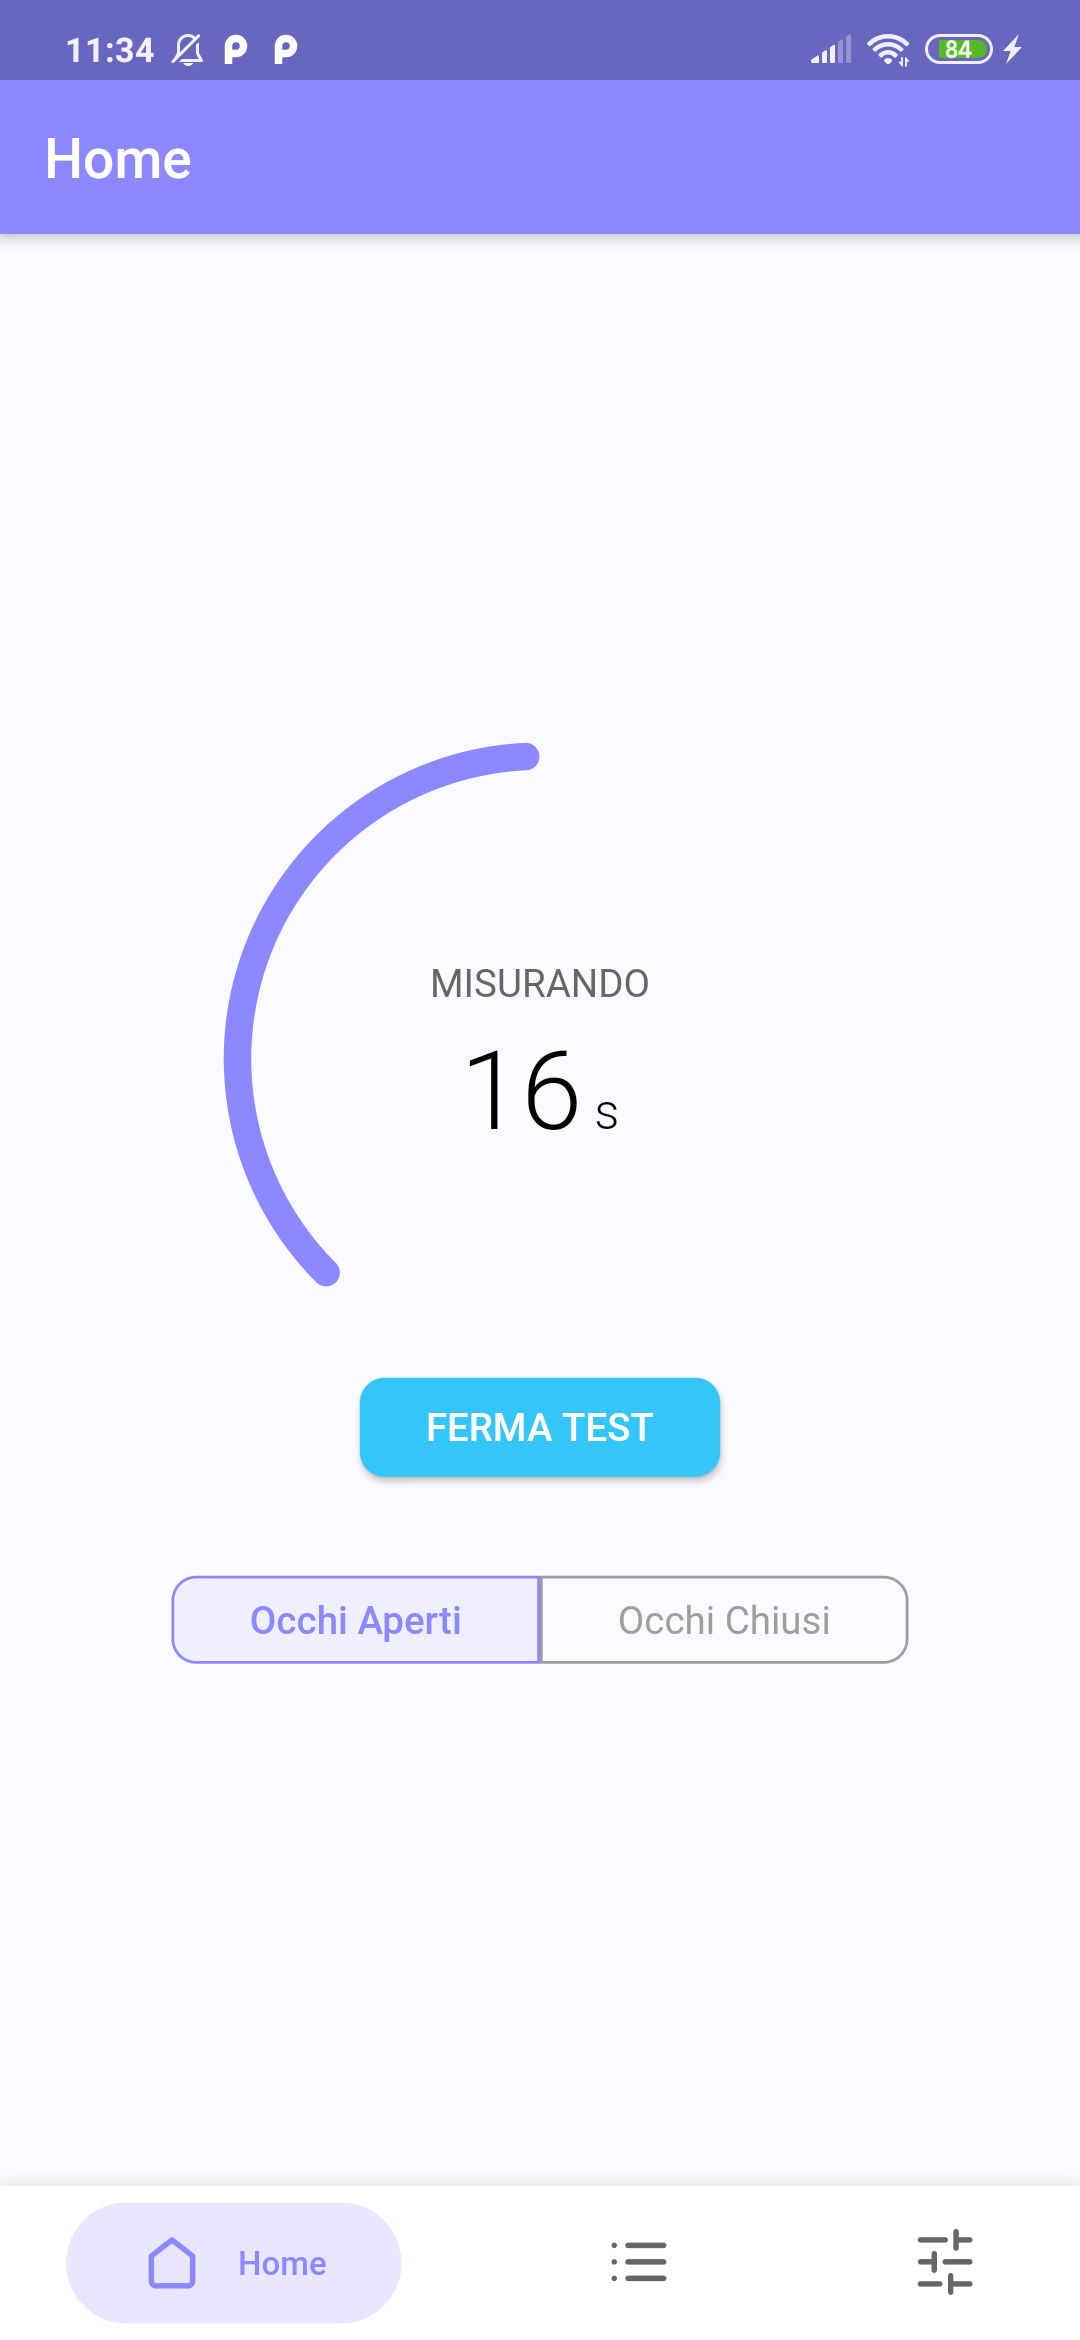
\includegraphics[width=\textwidth]{figures/screenshot/redmi_note_8t/home_measuring.png}
        \caption{durante la misurazione}
        \label{fig:home_measure}
    \end{subfigure}
    \caption{Schermata Home}
\end{figure}

\subsection{test eseguiti in precedenza}
L'utente può consultare lo storico di tutti i test eseguiti nell'apposita pagina (Figura \ref{fig:measurements}), qui ogni test è elencato sotto forma di lista ordinata per data di creazione.

\begin{figure}[!htb]
    \centering
    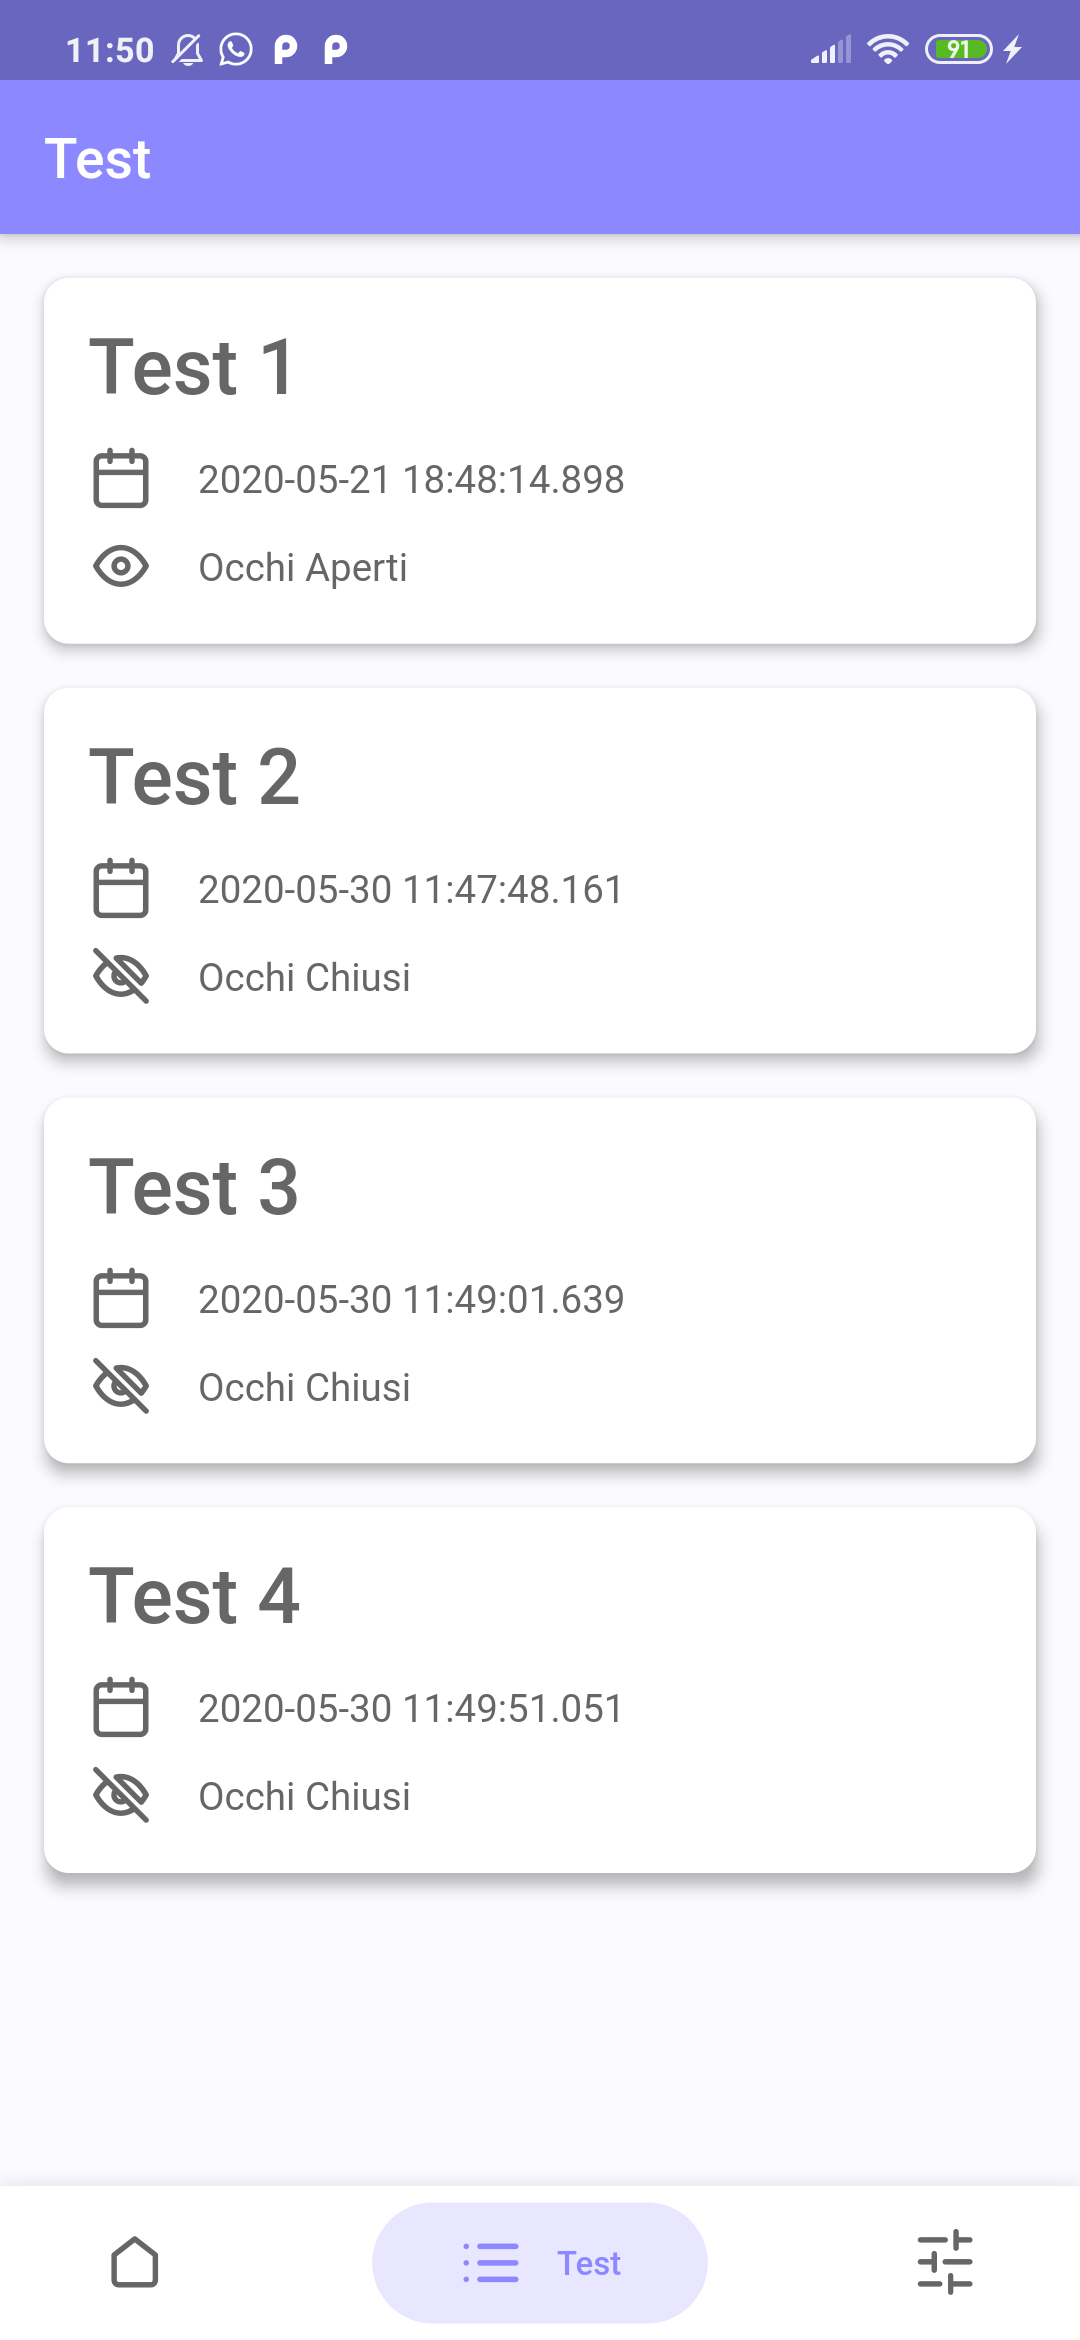
\includegraphics[width=.32\textwidth]{figures/screenshot/redmi_note_8t/measurtements.png}
    \caption{Schermata con i vecchi test}
    \label{fig:measurements}
\end{figure}

\subsection{impostazioni}
Qui l'utente può accedere a diverse pagine tra le quali: la calibrazione del dispositivo, il riepilogo dei dati personali, le informazioni riguardo le dipendenze utilizzate e maggiori informazioni sull'applicazione (Figura \ref{fig:settings}).

\begin{figure}[!htb]
    \centering
    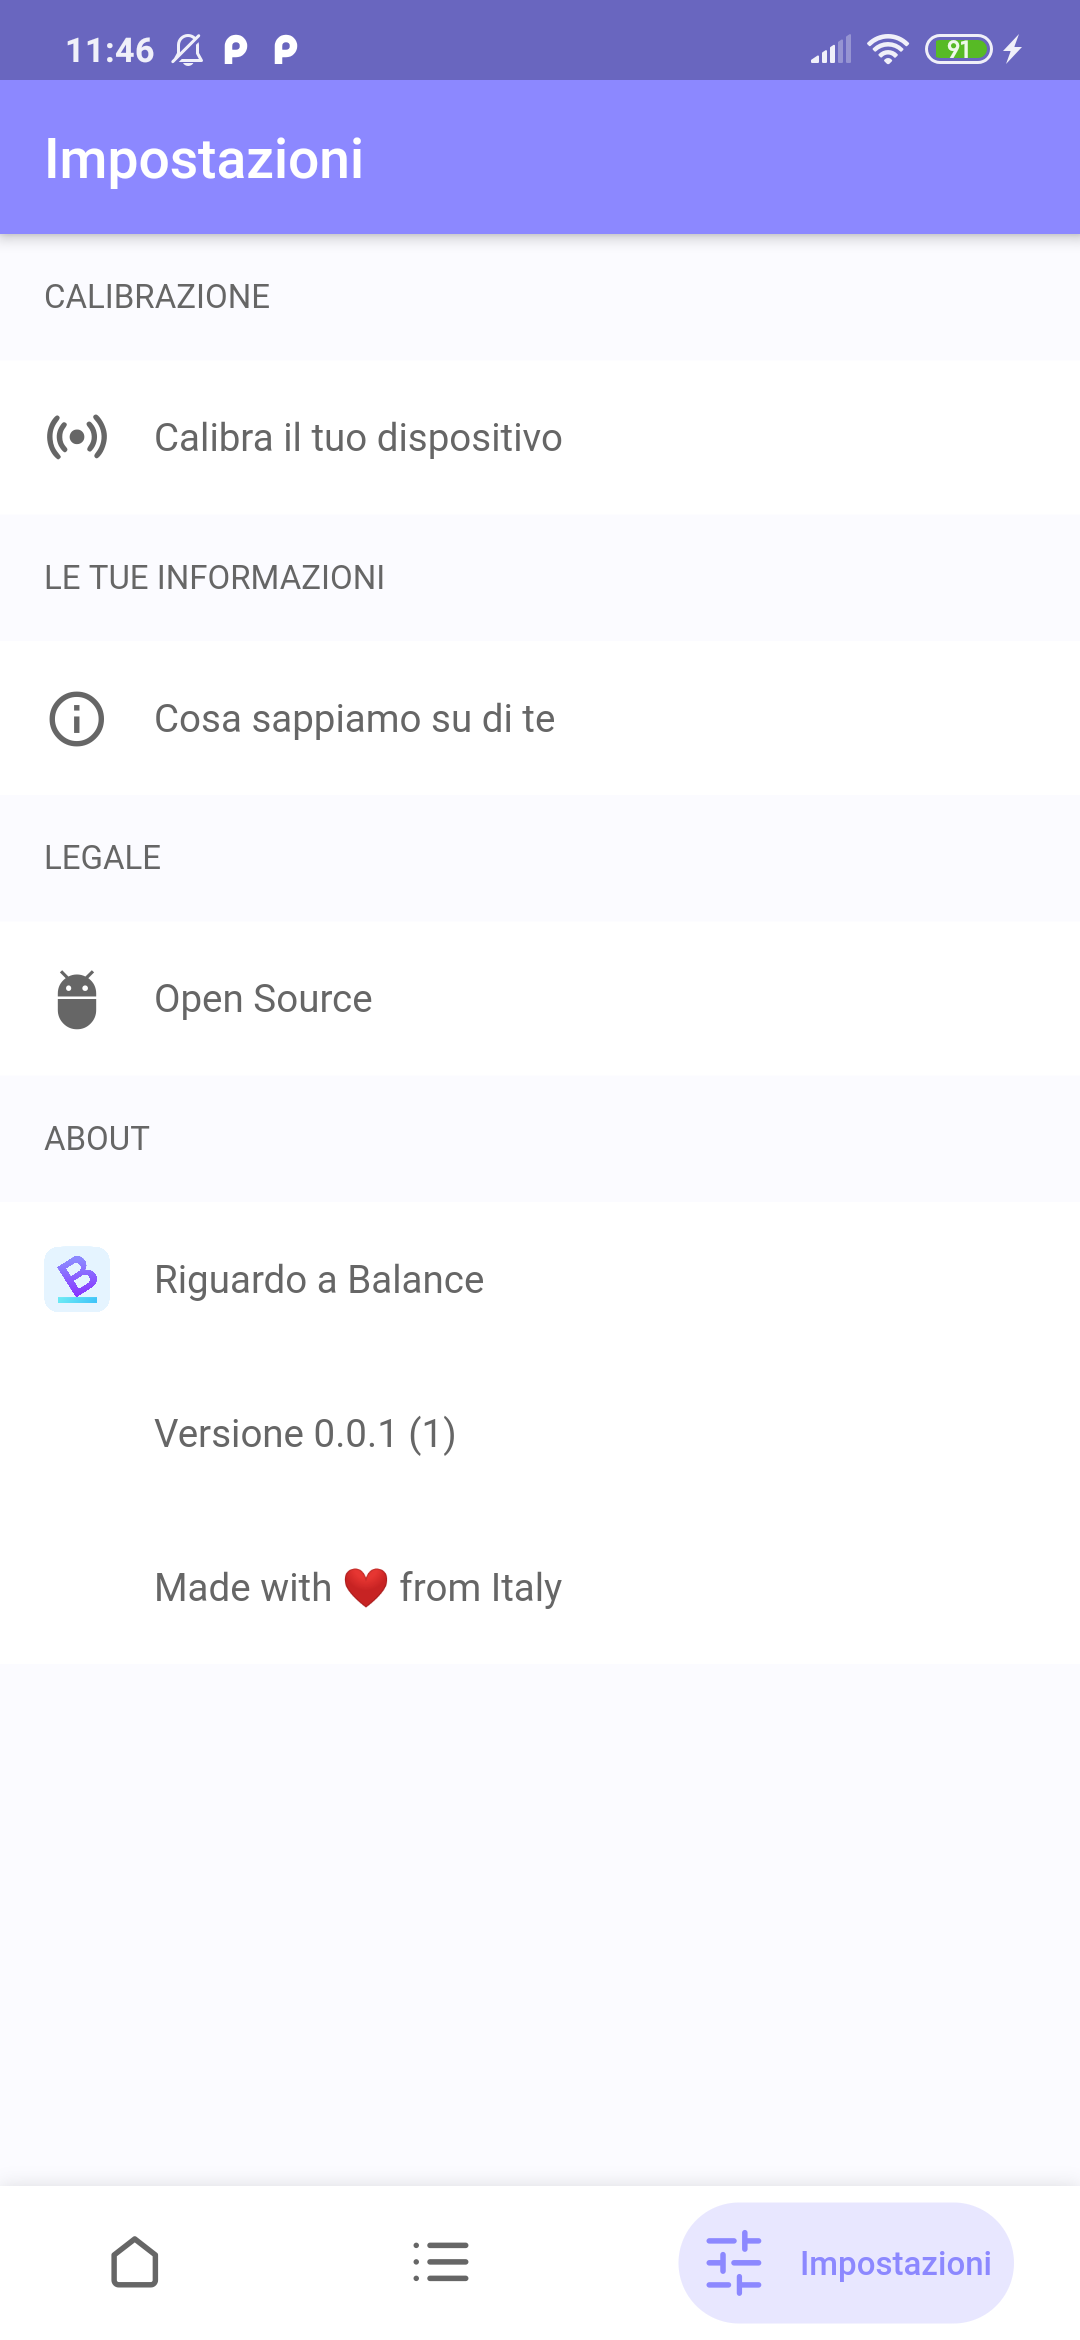
\includegraphics[width=.32\textwidth]{figures/screenshot/redmi_note_8t/settings.png}
    \caption{Schermata delle impostazioni}
    \label{fig:settings}
\end{figure}

\subsection{calibrazione del dispositivo}
Per regolare l'accuratezza dei sensori, rimuovendo eventuali errori nella taratura di fabbrica o difetti di produzione, l'utente è tenuto almeno una volta ad eseguire la calibrazione del proprio smartphone ed è proprio in questa schermata (Figura \ref{fig:c}) che viene eseguita. Premendo il bottone {\bfseries Inizia Calibrazione} si dà inizio al processo di calibrazione della durata di 10 secondi (Figura \ref{fig:ca}).

\begin{figure}[!htb]
    \centering
    \begin{subfigure}{.4\textwidth}
        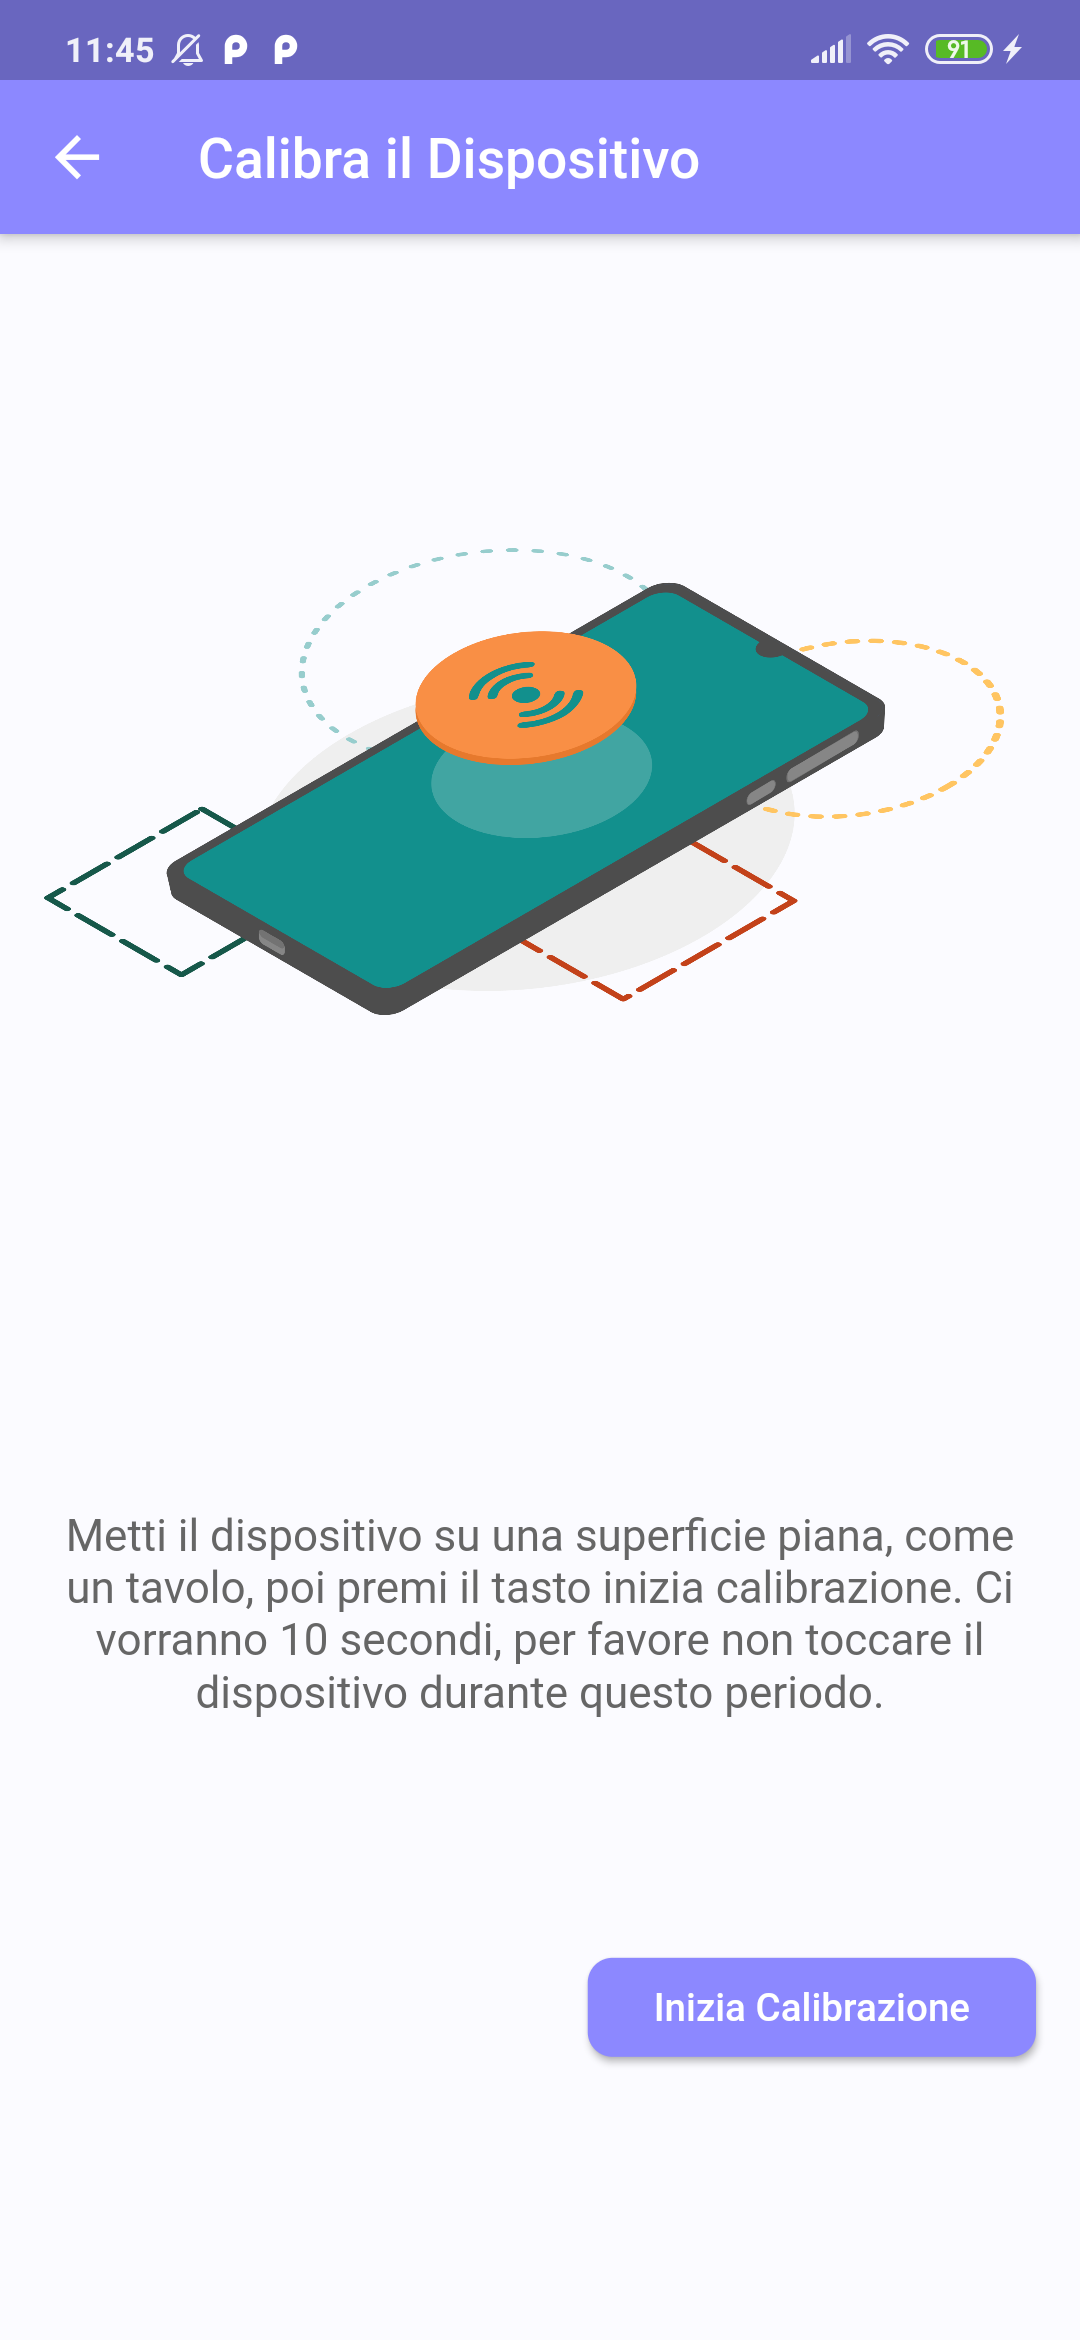
\includegraphics[width=\textwidth]{figures/screenshot/redmi_note_8t/calibrate.png}
        \caption{allo stato normale}
        \label{fig:c}
    \end{subfigure}
    \begin{subfigure}{.4\textwidth}
        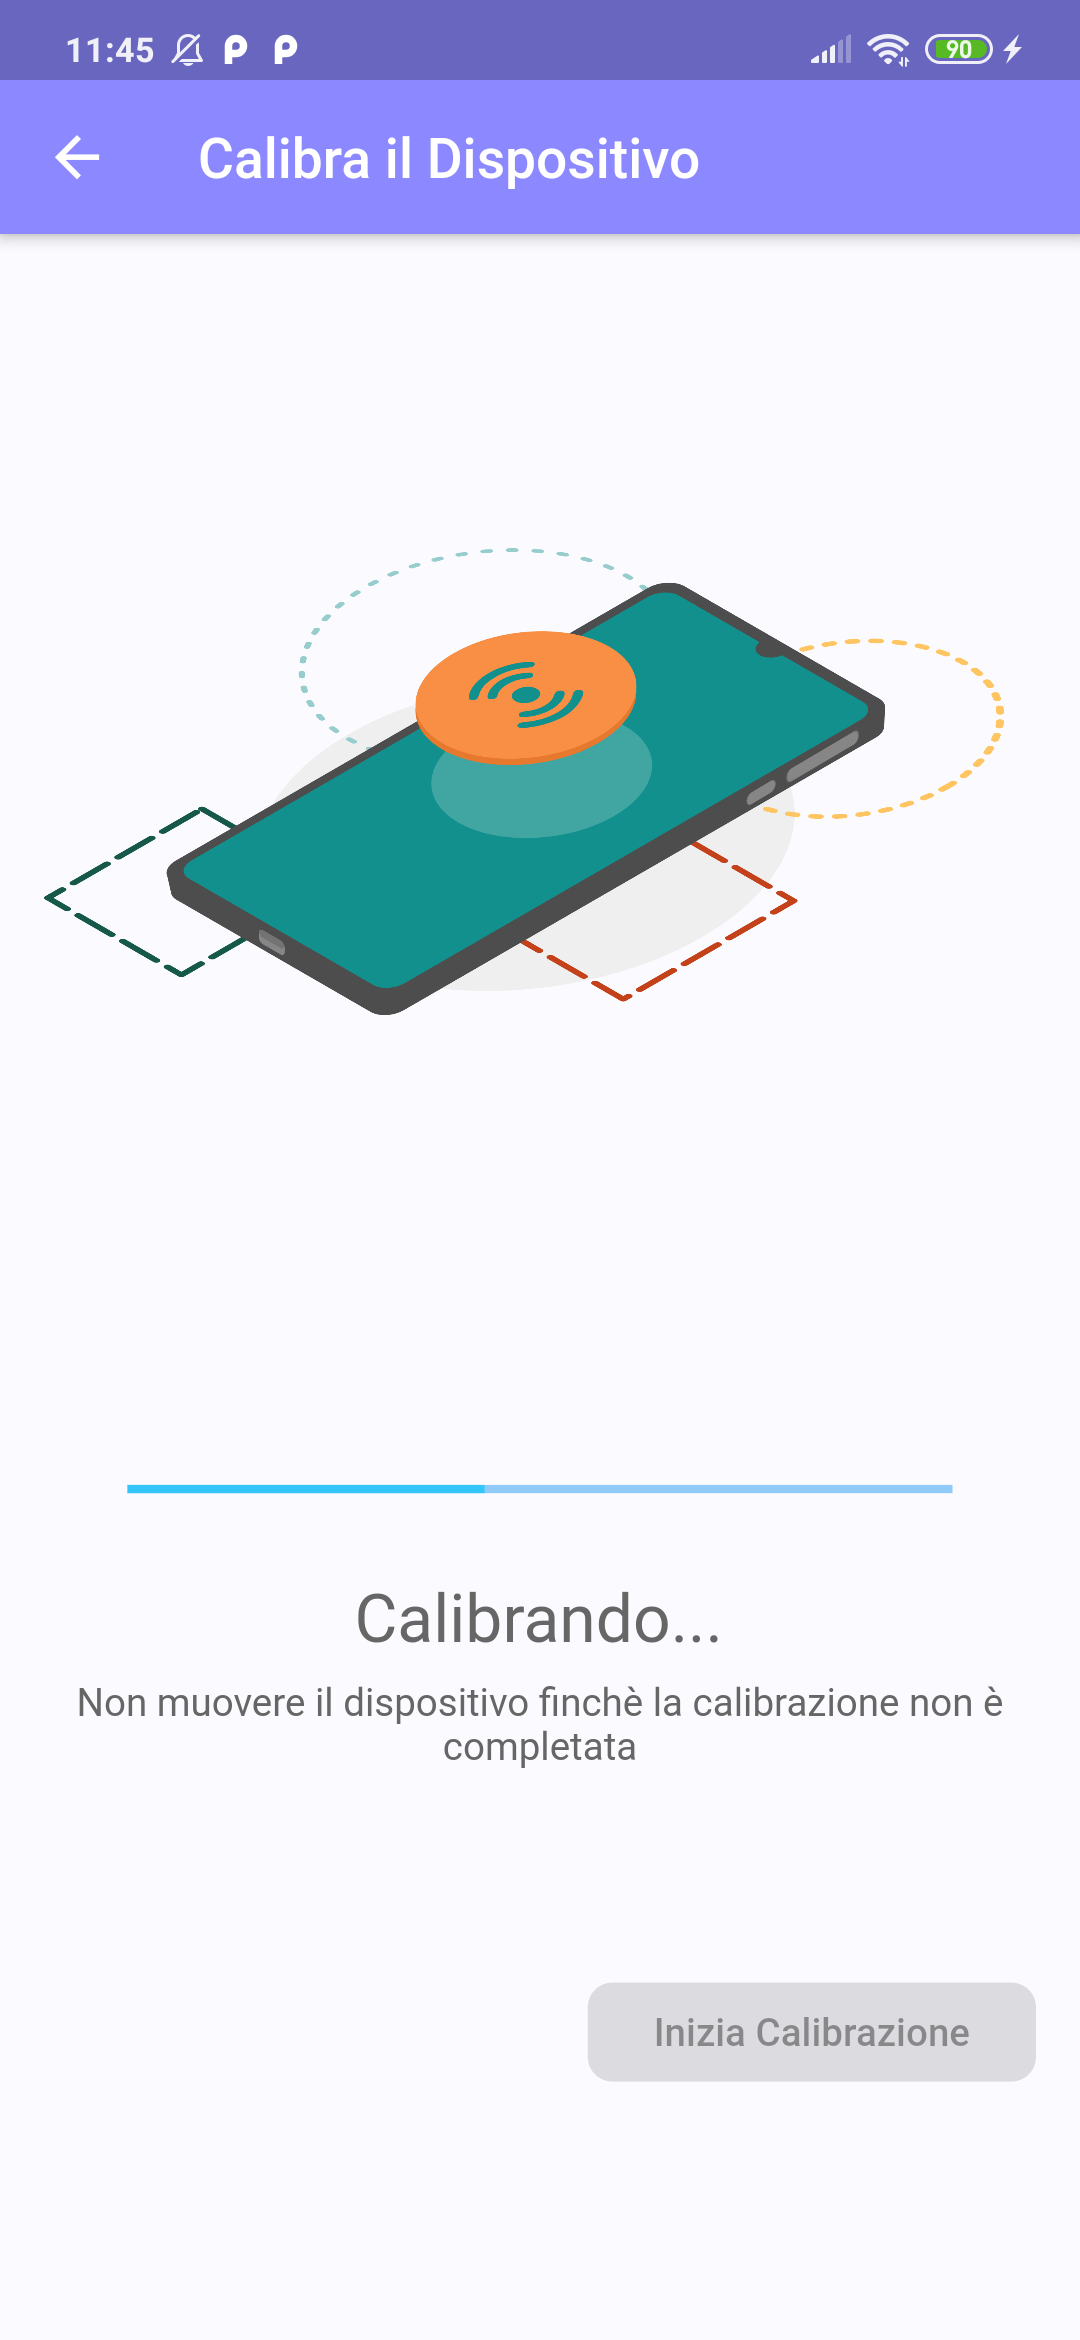
\includegraphics[width=\textwidth]{figures/screenshot/redmi_note_8t/calibrating.png}
        \caption{durante la calibrazione}
        \label{fig:ca}
    \end{subfigure}
    \caption{Schermata di calibrazione del dispositivo}
\end{figure}

\subsection{riepilogo dei dati personali}
In questa schermata è possibile vedere il riepilogo di tutti i dati d'anamnesi inseriti durante il primo avvio (Figura \ref{fig:info}), inoltre è possibile modificarli, premendo sul bottone con l'icona a forma di matita posto in basso, così facendo si verrà riportati nelle schermate di onboarding solo che questa volta i campi saranno precompilati con i dati inseriti in precedenza e sarà quindi possibile modificarli (Figura \ref{fig:precompiled}).

\begin{figure}[!htb]
    \centering
    \begin{subfigure}{.4\textwidth}
        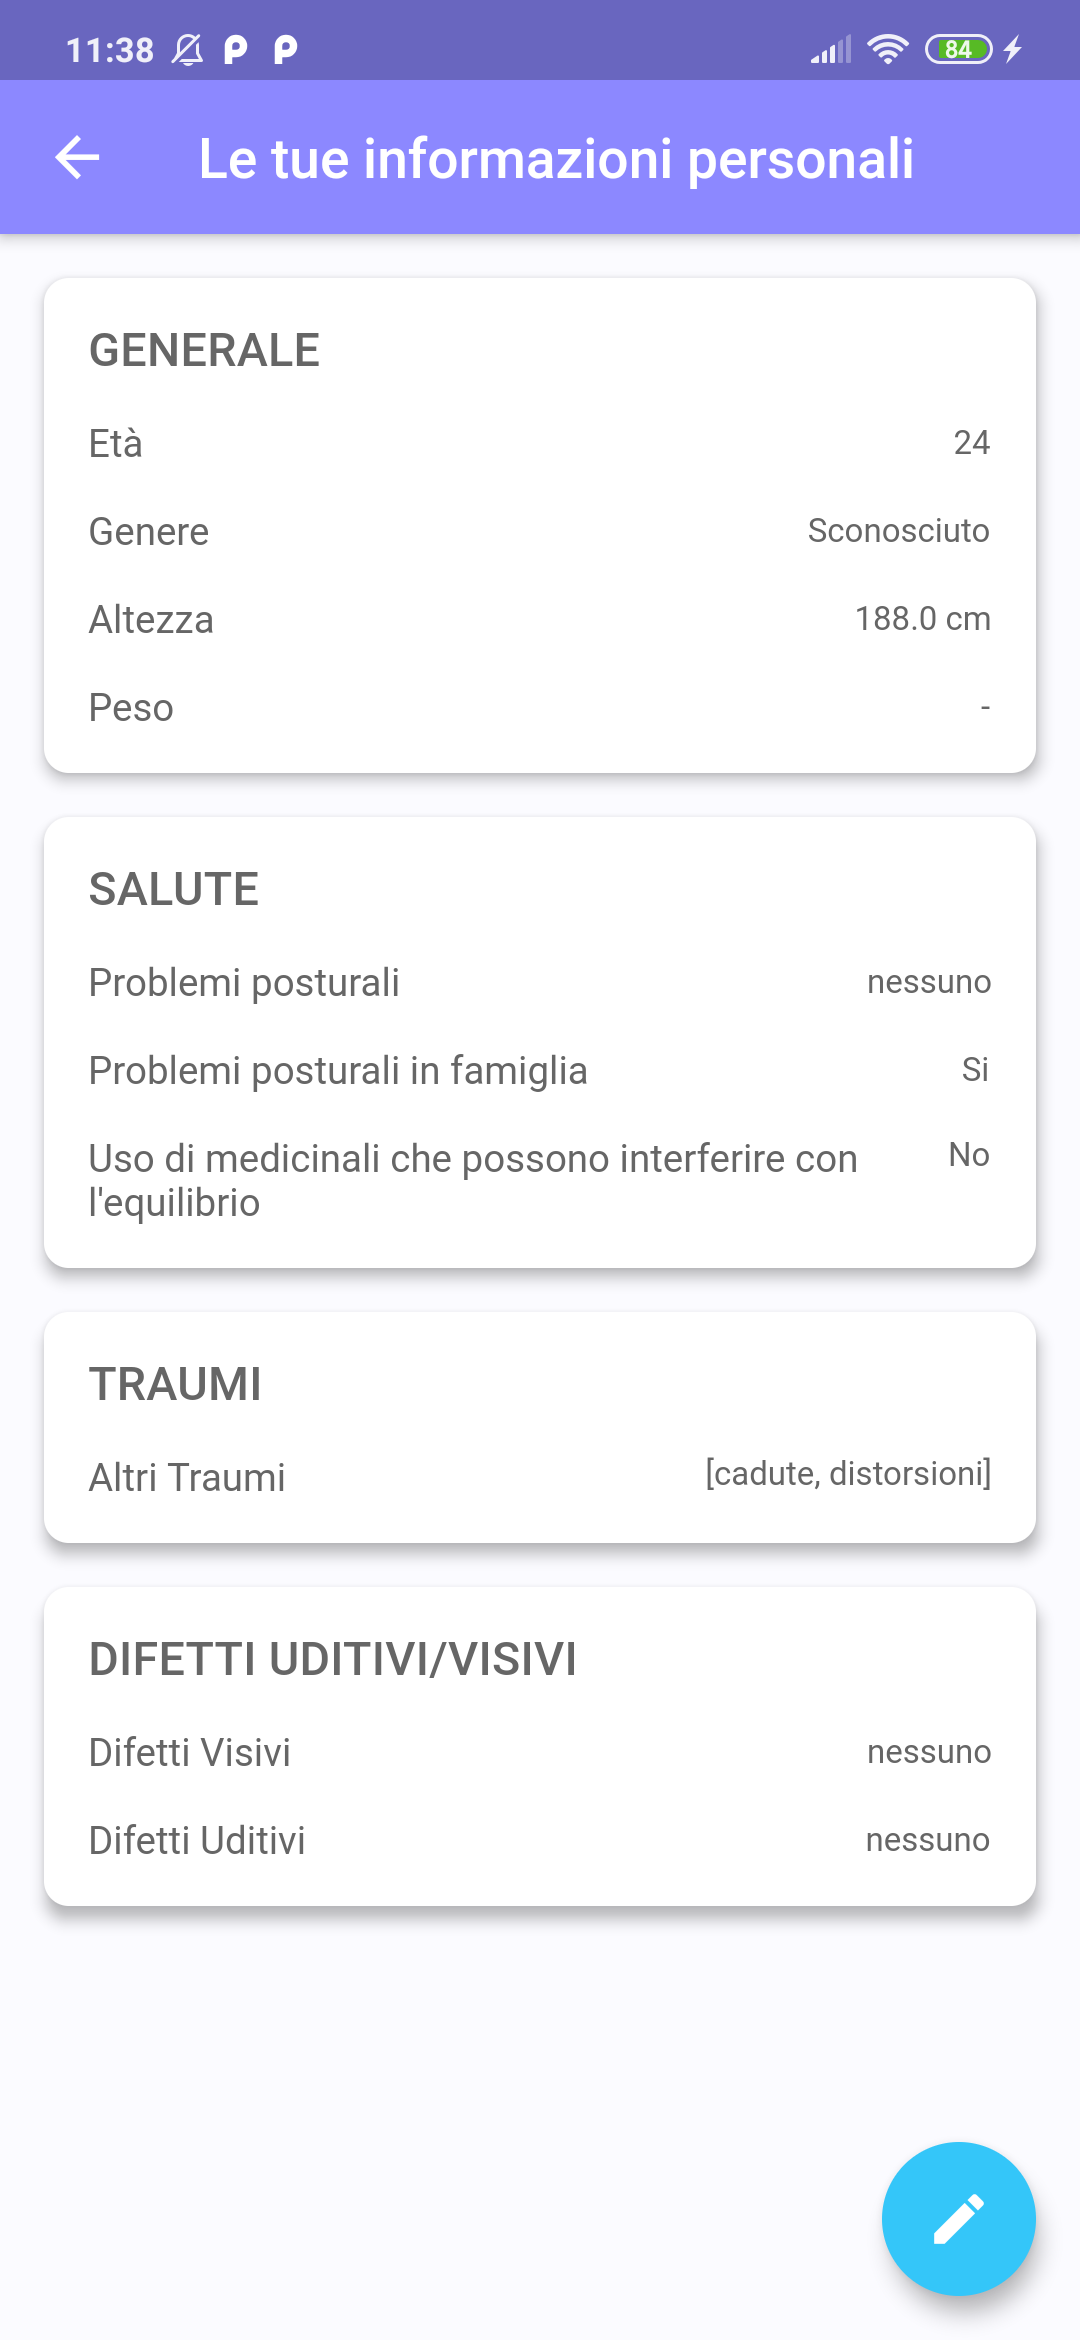
\includegraphics[width=\textwidth]{figures/screenshot/redmi_note_8t/your_info.png}
        \caption{riepilogo dei dati d'anamnesi}
        \label{fig:info}
    \end{subfigure}
    \begin{subfigure}{.4\textwidth}
        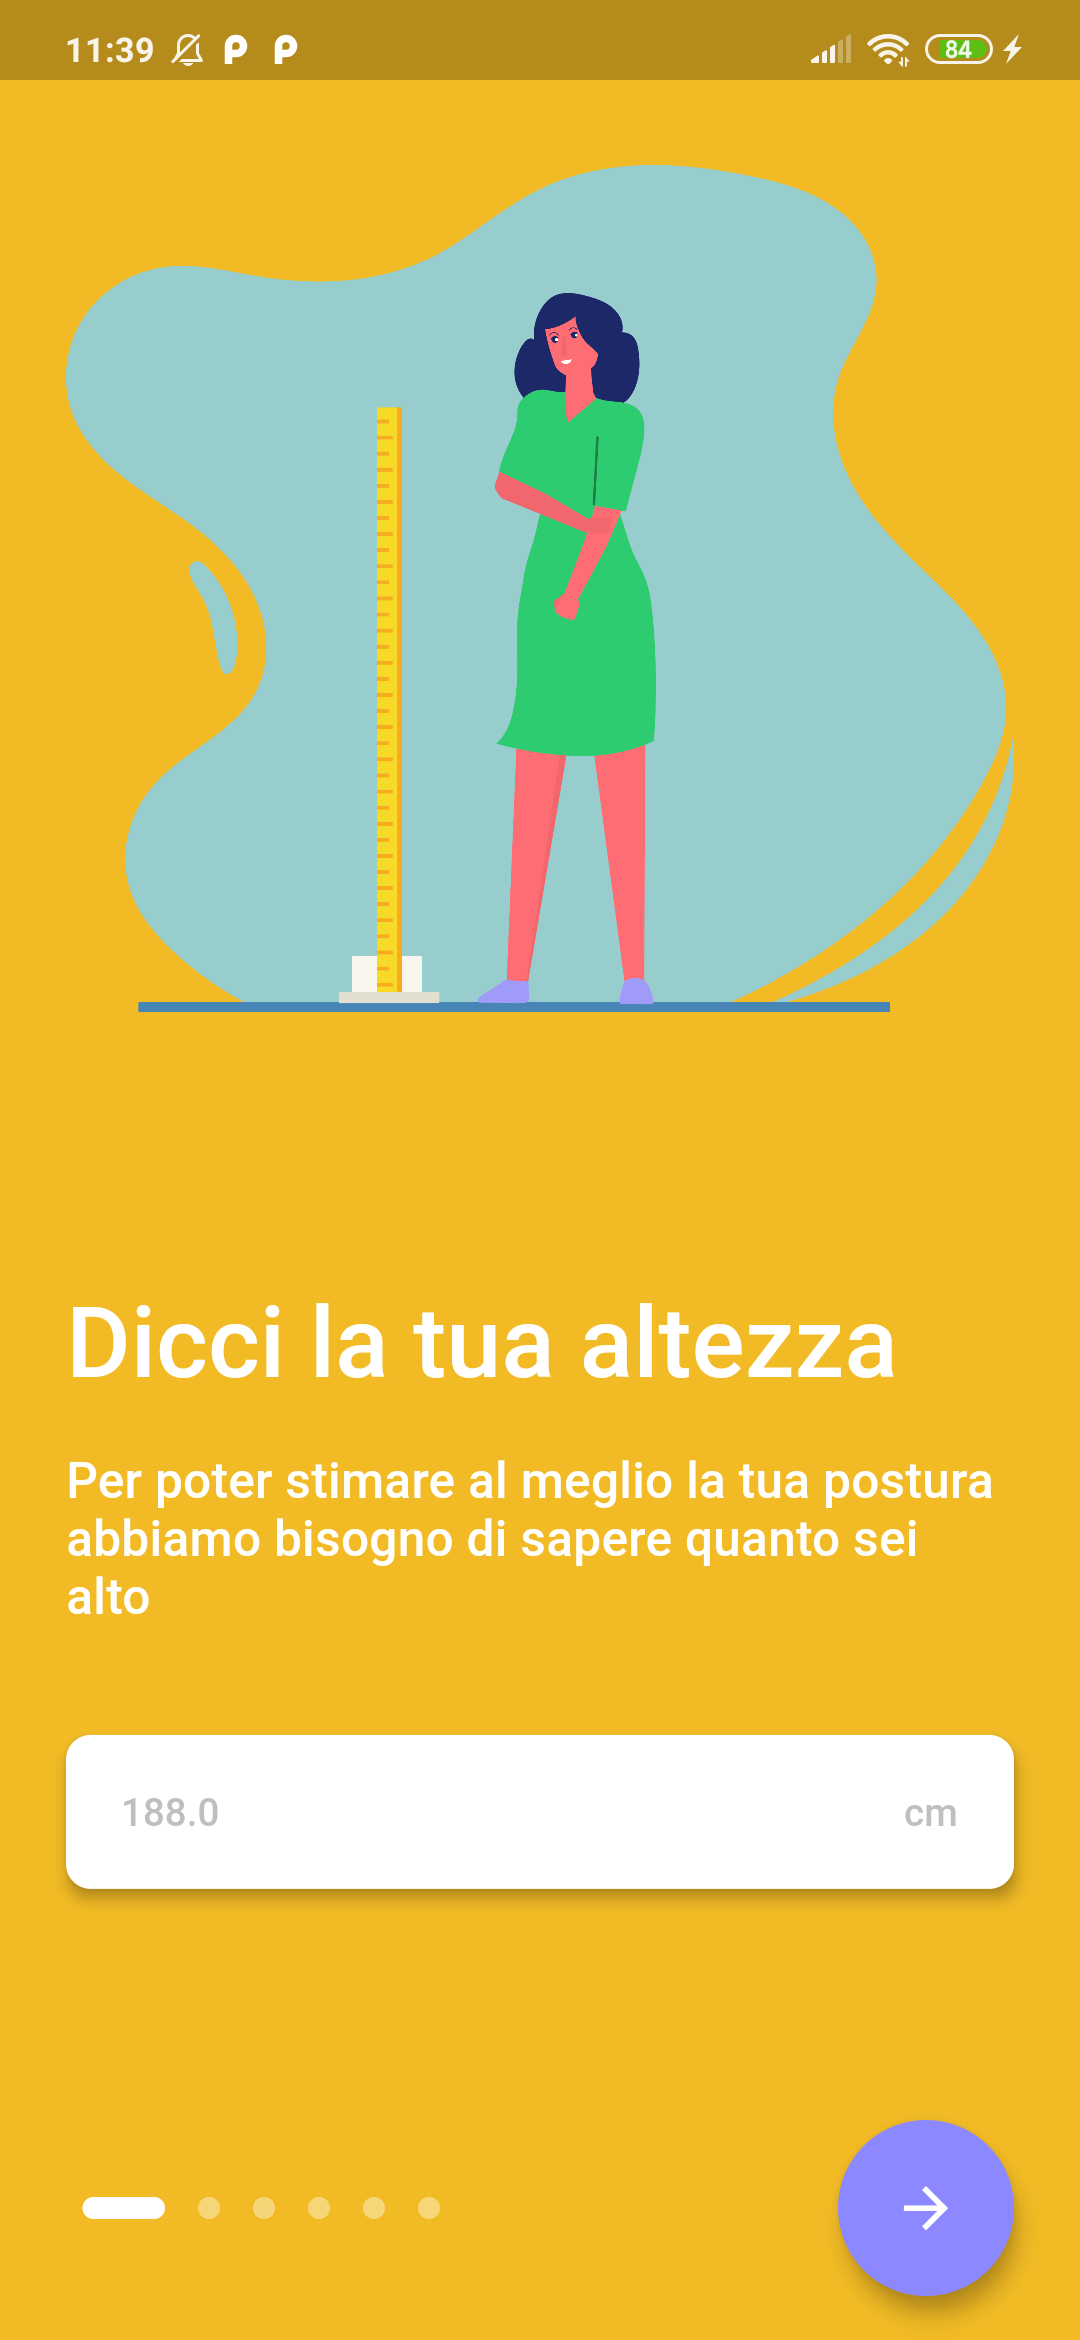
\includegraphics[width=\textwidth]{figures/screenshot/redmi_note_8t/height_precompiled.png}
        \caption{modifica dei dati d'anamnesi}
        \label{fig:precompiled}
    \end{subfigure}
    \caption{Riepilogo dei dati d'anamnesi inseriti durante il primo avvio}
\end{figure}

\subsection{risultati di un test}
Lo scopo di questa schermata è mostrare all'utente i risultati prodotti da un determinato test; l'intera pagina è raggruppata in diverse sezioni (Figura \ref{fig:result}): la prima card contiene le informazioni generali sul test (data in cui è stato effettuato e se era ad occhi aperti oppure chiusi); nella seconda sono inseriti i grafici di statokinesigramma e stabilogramma, nelle restanti sono elencati i valori delle features viste nel Capitolo \ref{cap:analisi_stabilometriche}.

\begin{figure}[!htb]
    \centering
    \begin{subfigure}{.4\textwidth}
        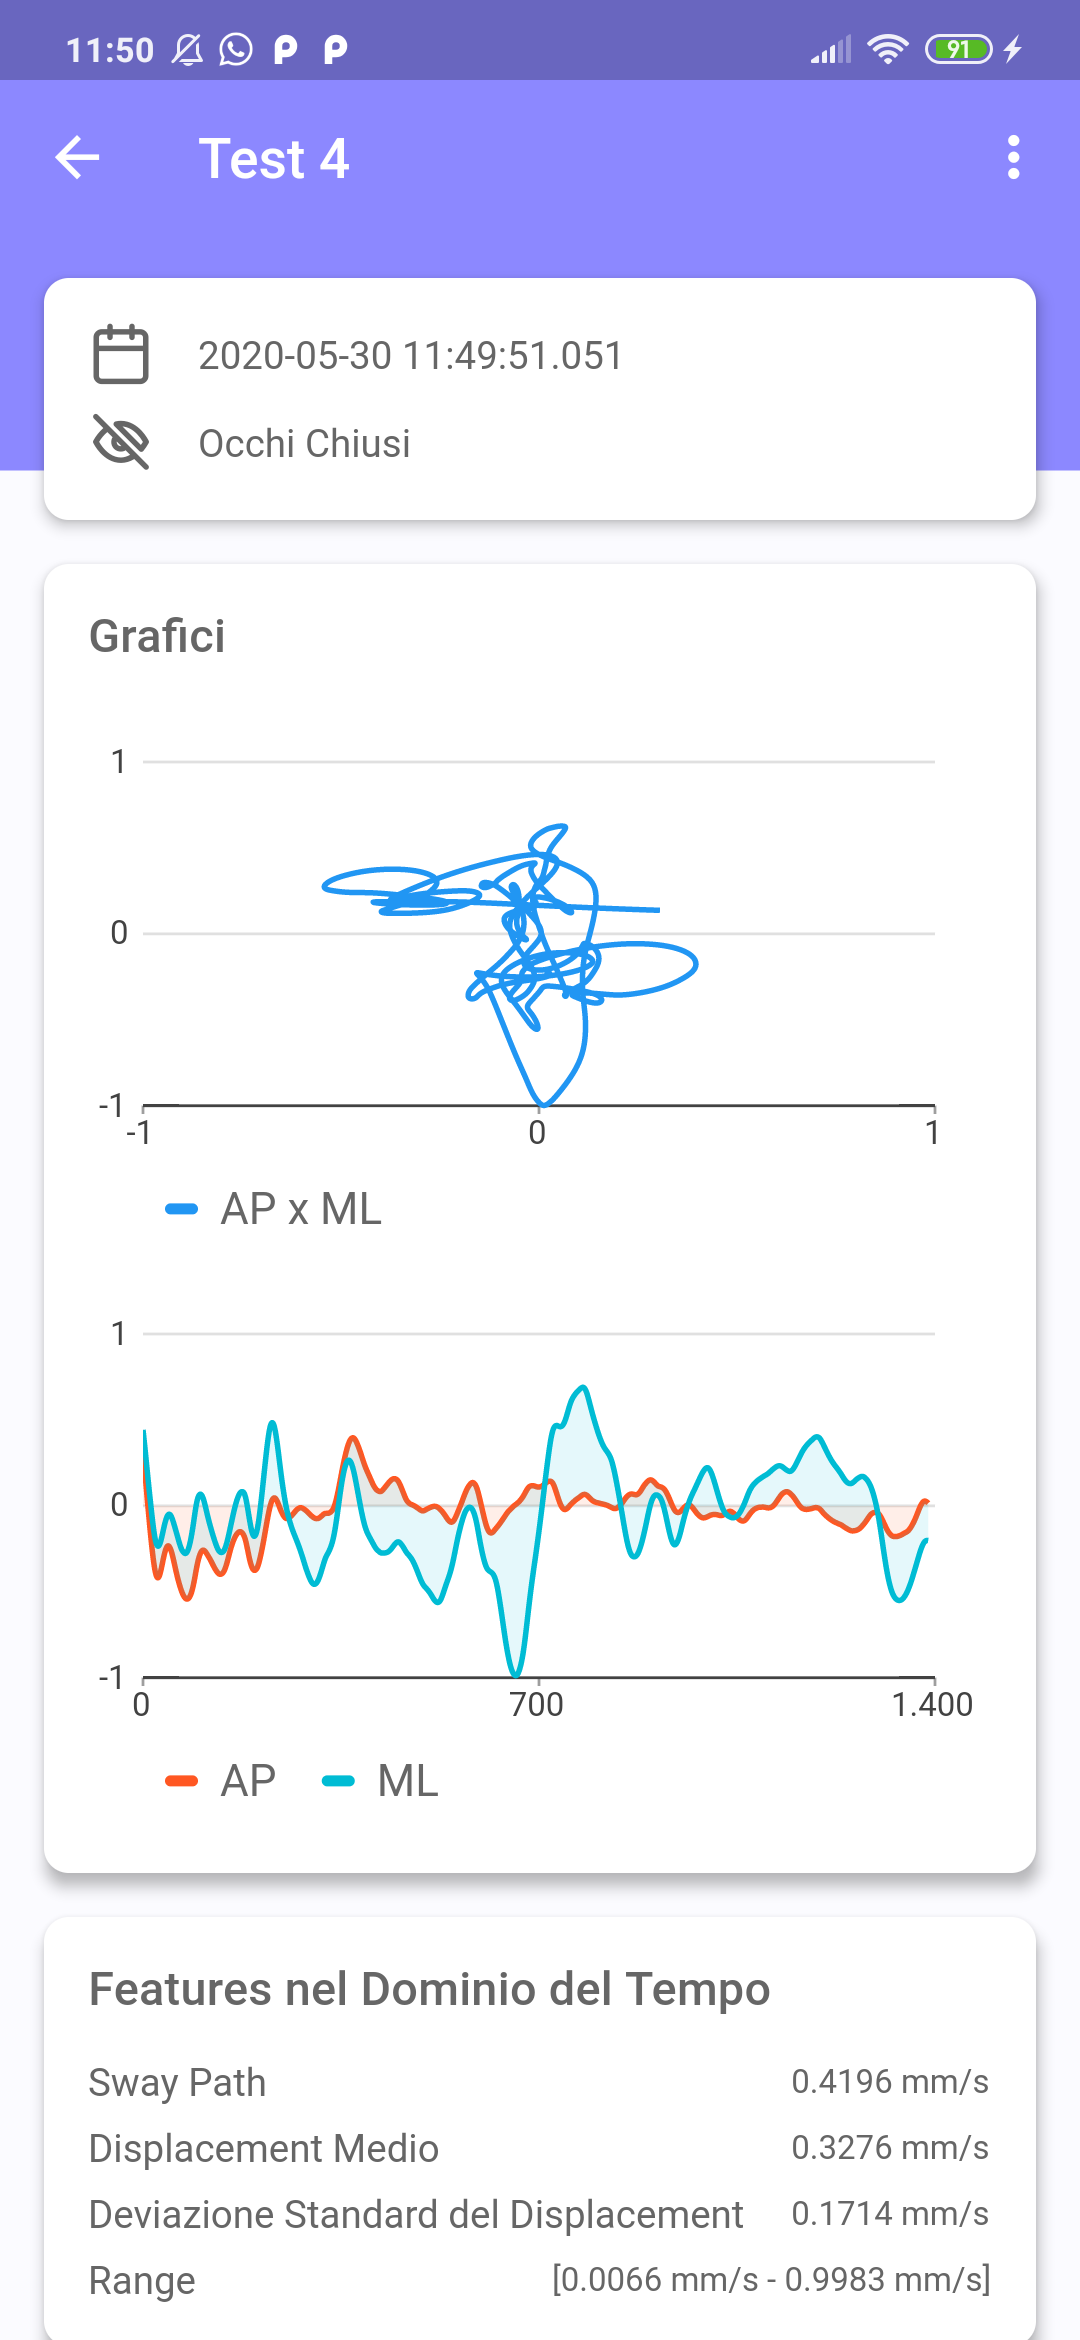
\includegraphics[width=\textwidth]{figures/screenshot/redmi_note_8t/result.png}
    \end{subfigure}
    \begin{subfigure}{.4\textwidth}
        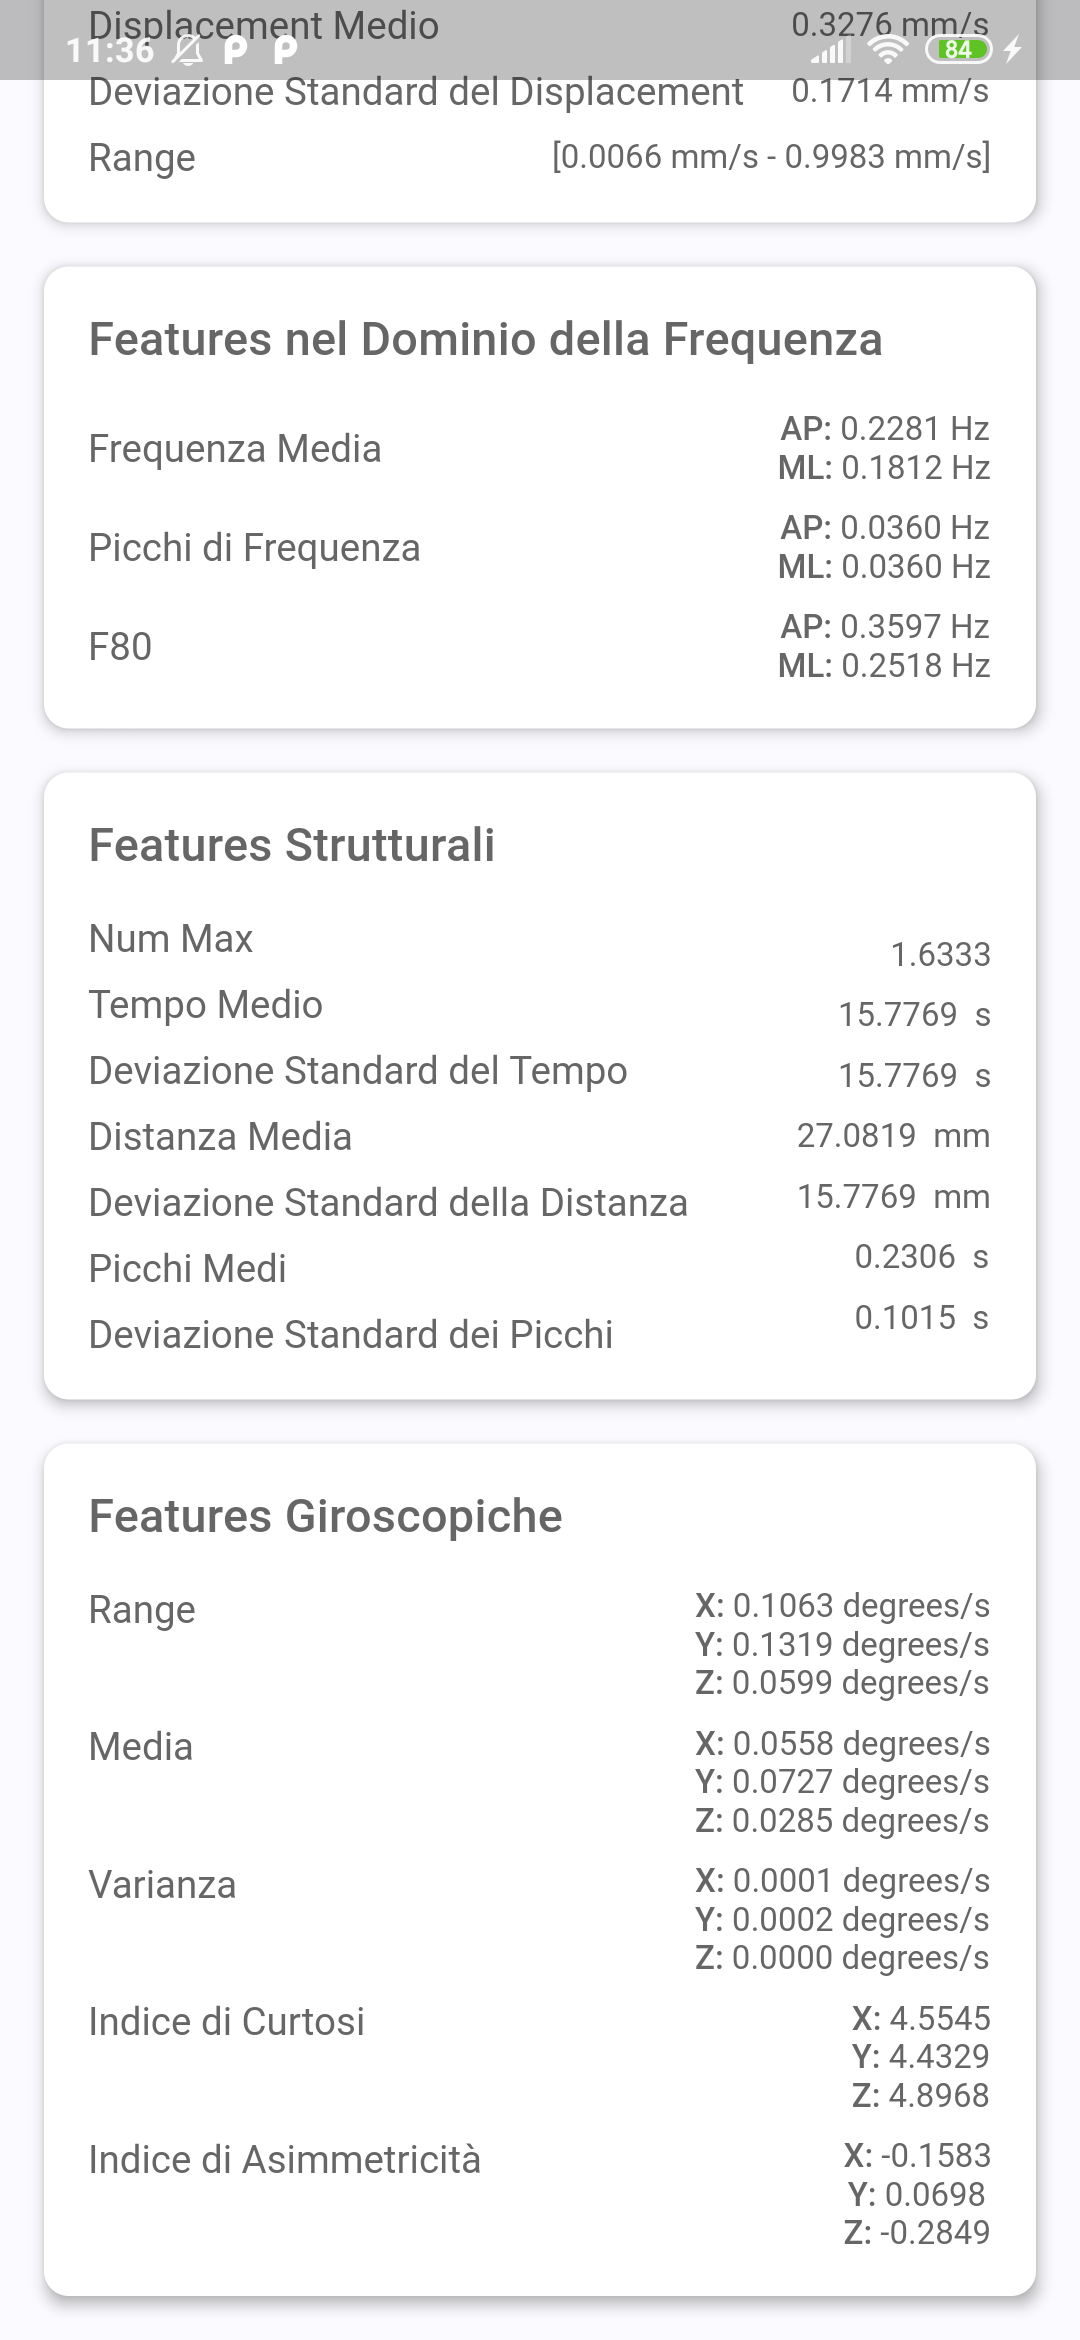
\includegraphics[width=\textwidth]{figures/screenshot/redmi_note_8t/result_bottom.png}
    \end{subfigure}
    \caption{Schermata con i risultati di un test}
    \label{fig:result}
\end{figure}

\section{Il database}

Internamente l'applicazione utilizza diversi metodi per salvare i dati a seconda del loro tipo. I valori dei sensori non elaborati, le features e le misure di stabilogramma sono contenuti in un database di tipo SQLite utilizzando le query SQL per manipolarli. I dati d'anamnesi, i bias dei sensori e diversi flag (flag per il primo avvio, flag per la calibrazione dei sensori, ecc) sono invece salvati come stringhe in coppie chiave-valore utilizzando le SharedPreferences in Android e NSUserDefaults in IOS. Questo meccanismo in futuro può essere facilmente esteso integrando un database ospitato su un server remoto che fa uso di un API Rest per gestire i dati e rappresenta ogni utente come un id univoco. Dal lato dell'applicazione l'integrazione è piuttosto semplice, la struttura interna rappresenta le basi di dati come delle repository astraendo la vera origine che può essere sia interna al dispositivo che remota.
\chapter{Conclusioni}
\label{cap:conclusioni}
In questa tesi è stata sviluppata un'applicazione multipiattaforma per smartphone in grado di valutare la postura dell'utente raccogliendo dati dai sensori presenti all'interno del dispositivo. Immaginando il corpo umano come un singolo pendolo inverso è stato possibile convertire la variazione dei valori misurati dall'accelerometro in variazioni del centro di gravità ($COG_v$), in questo modo non è stato complesso ricavare i grafici di stabilogramma e statokinesigramma; dalla variazione del centro di gravità, inoltre, sono estratti i valori delle features studiando il segnale nel dominio del tempo e in quello della frequenza.

Come detto in precedenza lo sviluppo per dispositivi IOS non è stato approfondito perciò in futuro potrebbe risultare interessante terminare il lavoro anche su questa piattaforma.

Fra i potenziali sviluppi futuri dell'applicazione sicuramente è presente l'integrazione di un database on-line in cui poter raccogliere le misurazione di ogni utente assieme ai dati d'anamnesi e ai valori calcolati. In questo ambito risulta di particolare interesse il rispetto delle nuove norme sulla privacy e il GDPR che obbliga gli sviluppatori a prestare più attenzione a quali dati vengono richiesti agli utenti e al modo in cui sono salvati. Per esempio ogni utente che utilizza il servizio può essere rappresentato solo da un identificativo generato casualmente ed ogni informazione fa riferimento solo a quello, per garantire il totale anonimato. Un altro ambito di progresso interessante può essere l'utilizzo di una struttura di back-end composta da micro-servizi con sistemi di backup dei dati automatici.

Infine un'ultima area di miglioramento è la richiesta dei dati d'anamnesi; per questa è opportuno uno studio più approfondito, magari, consultando il parere di vari esperti in modo da delineare un gruppo maggiore di informazioni che possono essere correlate a problemi posturali. In questo ambito esistono numerose opportunità di ricerca svolgendo un lavoro di correlazione fra tutti i dati richiesti e i valori estratti dalle misurazioni utilizzando persino nuove tecnologie come ad esempio il machine learning.

\begin{thebibliography}{9}

\bibitem{rubenstein}
L.Z. Rupenstein,
{\em Falls in older people: epidemiology, risk factors and strategies for prevention},
Age and Aging 35 (suppl\_2) ii37-ii41,
\url{doi:10.1093/ageing/afl084},
\url{https://academic.oup.com/ageing/article/35/suppl_2/ii37/15775},
2006.

\bibitem{krupitzer}
C. Krupitzer, T. Sztyler, J. Edinger, M. Breitbach, H. Stuckenschmidt, C. Becker,
{\em Hips Do Lie! A Position-Aware Mobile Fall Detection System},
2018 IEEE International Conference of Pervasive Computing and Communication (PerCom),
pp. 1-10,
\url{doi:10.1109/PERCOM.2018.8444583},
2018.

\bibitem{gillespie}
L.D. Gillespie, M.C. Robertson, W.J. Gillespie, C. Sherrington, S.Gates, L.M. Clemson, S.E. Lamb,
{\em Interventions for preventing falls in older people living in the community},
Cochrane Database of Systematic Reviews (9),
\url{doi:10.1002/14651858.CD007146.pub3},
\url{https://www.cochranelibrary.com/cdsr/doi/10.1002/14651858.CD007146.pub3/abstract},
2009.

\bibitem{mancini}
M. Mancini, F.B. Horak,
{\em The relevance of clinical balance assessment tools to differentiate balance deficits},
European journal of physical and rehabilitation medicine 46 (2),
239-248,
\url{https://www.ncbi.nlm.nih.gov/pmc/articles/PMC3033730}
2010.

\bibitem{roeing}
K.L. Roeing, K.L. Hsieh, J.J. Sosnoff,
{\em A systematic review of balance and fall risk assessment with phone technology},
Archives of Gerontology and Geriatrics 73,
222-226,
\url{doi:10.1016/j.archger.2017.08.002},
\url{http://www.sciencedirect.com/science/article/pii/S0167494317302698}
2017.

\bibitem{fitzpatrick93}
Fitzpatrick, R., McCloskey, D.I.,
{\em The perception of sway during standing in humans},
J. Physiol.: 478, 173-176,
1993.

\bibitem{konradson96}
Konradson, L., Raun, J.B., Sorensen, A.J.,
{\em Proprioception at the ankle: the effect of anaesthetic blockade of ligament receptors},
J. Bone Joint Surg. Br: 75B, 433-436,
1993.

\bibitem{kavounoudias98}
Kavounoudias, A., Roll, R., Roll, J.P,
{\em The plantar sole is a 'dynamometric map' for human balance control},
NeuroReport: 9, 3247-3252,
1998.

\bibitem{wu97}
Wu, G., Chiang, H.J.,
{\em The significance of somatosensory stimulations to the human foot in the control of postural reflexes},
Exp Brain Res.: 114, 163-169,
1997.

\bibitem{sensors}
Flutter,
{\em Flutter plugin for accessing the Android and iOS accelerometer and gyroscope sensors},
v0.4.2,
\url{https://pub.dev/packages/sensors},
2020

\bibitem{cudropdown}
L. Calisti,
{\em A simple dropdown library with custom style},
v0.0.1,
\url{https://pub.dev/packages/custom_dropdown},
2020.

\bibitem{iirjdart}
L. Calisti,
{\em An IIR filter library written in Dart. Highpass, lowpass, bandpass and bandstop as Butterworth, Bessel and Chebyshev Type I/II},
v0.0.1,
\url{https://pub.dev/packages/iirjdart},
2020.

\bibitem{powerdart}
L. Calisti,
{\em Compute the Power Spectral Density (PSD) on Dart. This package runs everywhere dart runs},
v0.0.2,
\url{https://pub.dev/packages/powerdart},
2020.

\bibitem{abtdependencies}
L. Calisti,
{\em Automatically generate dart file with informations about used dependencies in pubspec.yaml},
v0.0.1,
\url{https://pub.dev/packages/about_dependencies},
2020.
\end{thebibliography}


\ringraziamenti
Vorrei ringraziare di cuore tutte le persone che mi hanno permesso di arrivare fin qui e di portare a termine questo lavoro di tesi.

Un ringraziamento speciale va al Prof. Lattanzi per i suoi indispensabili consigli, per le conoscenze trasmesse e per la sua infinita disponibilità in ogni passo della realizzazione dell'elaborato, fin dalla scelta dell'argomento.

Ringrazio infinitamente la mia famiglia, senza i loro insegnamenti e senza il loro supporto, questo lavoro di tesi non esisterebbe nemmeno.

Ringrazio tutti i miei amici per essere stati sempre presenti anche durante quest'ultima fase del mio percorso di studi.

Infine, dedico questa tesi a me stesso, ai miei sacrifici e alla mia tenacia che mi hanno permesso di arrivare fin qui.

\end{document}
